\chapter{Introduction}
For the past twenty years Functional Magnetic Resonance Imaging (FMRI) 
has been at the forefront of cognitive research. Despite it's
limited temporal resolution, FMRI is the standard tool for localizing 
neural activation.  Whereas other methods
of analyzing neural signals can be invasive or difficult to acquire, 
FMRI is relatively quick and cheap, and its analysis relatively straight forward.

By modeling the governing equations behind the neural response that
drives FMRI, it is possible to make the analyses of FMRI even more
powerful. The underlying state equations hold important information
about how individual brain regions react to stimuli. The model parameters
on the other hand, hold important information about the patients individual
physiology including existing and future pathologies. In short,
the long chain of events driving observable FMRI signal contains more
information than which regions respond to which stimuli.

In the past fifteen years, a steady stream of studies have built
on the original Blood Oxygen Level Dependent (BOLD) signal 
derivation first described by \cite{Ogawa}.
The seminal work by \cite{Buxton1998} attempted to explain the
time evolution of the BOLD signal using a windkessel model to
describe the time local changes in Deoxygenated Hemoglobin content.
Various papers made substantial improvements to this model until
\cite{Buxton2004} brought all the changes together into a single complete 
set of equations. And while there have been numerous adaptations in the model, 
many of them summarized in \cite{Deneux2006}, even the most basic version
has been shown to have less bias error than the convolution based 
"Canonical Hemodynamic Model" \cite{Deneux2006}, \cite{Handwerker2004}.
On the other hand many of the BOLD signal models have far more parameters
than a simple scaling parameter. In fact, the number of parameters
range from seven \cite{Riera2004} to 50 \cite{Behzadi2005} per
signal time course; a signal which may be as short as 100 samples long.
Thus, even in a small FMRI image of the brain (20x20x20), the number of parameters 
could easily exceed 10,000. Clearly this number of parameters presents
a significant risk of being under-determined and could suffer catastrophic
variance error; to make no mention of the computation cost. 
In this work a method of countering these problem is presented
with the use of a particle filter.

\section{Overview}
\label{sec:Introduction Overview}
Detecting neural activity using the changes in FMRI images is based on 
the so called Blood Oxygen Level Dependent (BOLD) signal.
The BOLD signal is caused by minute changes in the ratio of Deoxygenated
Hemoglobin to Oxygenated Hemoglobin in blood vessels throughout the brain.
Because Deoxygenated Hemoglobin (DHb) is paramagnetic, higher concentrations
attenuate the signal detected during T2-weighted Magnetic Resonance Imaging (MRI)
techniques. The most common FMRI imaging technique, due to its rapid repetition 
time (TR), is Echo Planar Imaging (EPI). When axons becomes active,
a large amount of ions quickly flow out of the cell. In order for this
action potential to occur again (and thus for the neuron to fire again),
an active pumping process must move ions back into the
axon. This process of recharging the axon requires extra energy, which temporarily
increases the metabolic rate of oxygen. On a massive scale (cubic millimeter) 
this activation/recharge process happens continuously. However, when a 
particular region of the brain is very active, the action potentials
occur significantly more often, resulting in significant local increase
of the 
Cerebral Metabolic Rate of Oxygen (CMRO2). Thus, blood vessels in a very 
active area will 
tend to have less oxygenated hemoglobin (due to the increased rate at which
oxygen is being consumed), and more deoxygenated hemoglobin,
resulting in an attenuated FMRI signal. In compensation for 
activation, muscles that
control blood vessels relax in that region to allow more blood flow,
which actually overcompensates.
This ultimately results in lower than average concentration of 
deoxyhemoglobin. Thus, the BOLD signal consists of a short initial
dip in the MR signal, followed by a prolonged increase in signal
that slowly settles out. It is this overcompensation that is the 
primary signal detected with FMRI imaging. This cascade of events
is believed to consist of increased the local metabolism, 
blood flow, blood volume, and oxygenated hemoglobin. The differences
in onsets of these various effects is what causes the overcompensation
that is observable in FMRI. Unfortunately, FMRI has no inherent unit
of measurement, and thus signal levels are all relative: within a particular
person, scanner and run. 

\section{FMRI}
Magnetic Resonance Imaging, MRI, is a method of building 3D images
non-invasively, based on the difference between nuclear spin
relaxation times in various molecules. First, the subject 
is brought into a large magnetic field which causes nuclear spins
to align. Radio Frequency (RF) signals may
then be used to excite nuclear spin away from the base alignment. 
As the nuclei precess back to the alignment of the magnetic
field, they emit detectable RF signals. Conveniently, the
excitation of nuclear spins return their original state at different
rates, called the T1 relaxation time, depending on the atoms excited.
Additionally, the
coherence of the spins also decay differently (and quite a bit faster
than T1 relaxation) based on the properties of the region.
This gives two primary methods of contrasting substances,
which form the basis of T1 and T2 weighted images. Additionally, 
dephasing occurs at two different rates, the T2 relaxation time,
which is unrecoverable, and T2$^*$ relaxation, which is
much faster, but possible to recover from via special RF signals.
T1 relaxation times are typically on the order of seconds if 
a sufficiently strong excitation was applied. 
In order to rapidly acquire entire brain images, as done in Functional 
MRI, a single large excitation pulse is applied to the entire brain,
and the entire volume is acquired in a single T1 relaxation period. 
Because the entire k-space (spatial-frequency) volume is acquired 
from a single excitation, the signal-to-noise-ratio is very low
in this type of imaging (Echo Planar Imaging). 

Increasing the spatial resolution of EPI imaging necessarily 
requires more time or faster magnetic field switching. Increasing
magnet switching rates though is difficult, because it can result in
more artifacts, or even lower signal to noise ratios. The result is
that at \emph{best} FMRI is capable of 1 second temporal resolution. 
The signal is further diluted because each voxel contains
the signal from a large number of neurons, capillaries and veins. 
Thus, the FMRI signal, which is sensitive to the chemical composition of 
materials, is the average signal from various types of tissue
in addition to the blood. As mentioned in \autoref{sec:Introduction Overview},
and explored in depth in \autoref{sec:BOLD Physiology},
the usefulness of FMRI comes from the discerning of changes in 
Deoxyhemoglobin/Oxyhemoglobin. Therefore, it is necessary to assume
that in the short term the only chemical changes will be in
capillary beds feeding neurons. In practice this may not be the case, for
instance near significant veins, and it may explain some of the
noise seen in FMRI imaging (see \autoref{sec:Introduction Noise}. 
Because MRI lacks units and certain
areas will have a higher base MR signal, all FMRI studies deal with
percent change from the base signal; rather than raw values. This
also removes most of the structural data which is not helpful 
in determining neural activity.

\section{BOLD Physiology}
\label{sec:BOLD Physiology}
It is well known that the two types of hemoglobin act as a contrast agents in 
EPI imaging
\cite{Buxton1998}, \cite{WEISSKOFF1994}, \cite{Ogawa}, however the connection
between Deoxyhemoglobin/Oxygenated Hemoglobin and neural activity is non-trivial. 
Intuitively, increased 
metabolism will increase Deoxyhemoglobin, however blood vessels are quick
to compensate by increasing local blood flow. Increased inflow, accomplished by loosening 
capillary beds, precedes increased outflow, driving increased 
blood storage capacity.
Since the local MR signal depends on the ratio of Deoxyhemoglobin to Oxygenated
Hemoglobin, increased volume of blood can effect this ratio if 
metabolism doesn't exactly match the increased inflow of oxygenated blood.
This was the impetus
for the ground breaking balloon model (\cite{Buxton1998}) and windkessel
model (\cite{Mandeville1999}). These works derive from first principals
the changes in deoxyhemoglobin ratio and volume of capillaries based on a given flow.
These were the first two attempts to quantitatively account for the shape of the 
BOLD signal as a consequence of the lag between the cerebral blood volume (CBV) 
and the inward cerebral blood flow (CBF). In fact \cite{Buxton1998} went so far as
to show that a simple, well chosen blood flow waveform coupled with a square 
wave cerebral metabolic rate of oxygen (CMRO2) curve, in the context of a balloon 
model, could fully account for the BOLD signal. 

Although \cite{Buxton1998} demonstrated that a well chosen flow waveform could 
explain most features of the BOLD signal, there was still a matter of proposing a
realistic waveform for the CBF and for the CMRO2. \cite{Friston2000} gave
a reasonable and simple
expression for CBF input,$f$, based on a flow inducing signal, $s$, 
in combination with the original balloon model
where $v$ is normalized cerebral blood volume (CBV), $q$ is the normalized
local deoxyhemoglobin/oxygenated hemoglobin ratio.
\begin{eqnarray}
\dot{s} &=& \epsilon u(t) - \frac{s}{\tau_s} - \frac{f - 1}{\tau_f} \\
\dot{f} &=& s\\
\dot{v} &=& \frac{1}{\tau_0}(f - v^\alpha)\\
\dot{q} &=& \frac{1}{\tau_0}(\frac{f(1-(1-E_0)^f)}{E_0} - \frac{q}{v^{1-1/\alpha}})
\label{eq:bold}
\end{eqnarray}
where $\epsilon$ is a neuronal efficiency term, $u(t)$ is a stimulus, and $\tau_f$, $\tau_s$
are both time constants, $E_0$ is the resting metabolic
rate and $\alpha$ is Grubb's parameter controlling the balloon model. 

This completed the basic balloon model, and was well summarized again
in \cite{Riera2003}.  \cite{Obata2004} refined the readout equation 
of the BOLD signal based on the
deoxyhemoglobin content (q) and local blood volume (v), resulting in the
final BOLD equation:
\begin{eqnarray}
y   &=& V_0((k_1 + k_2)(1-q) - (k_2 + k_3)(1-v))\\
k_1 &=& 4.3 \times \nu_0 \times E_0 \times TE = 2.8\\
K_2 &=& \epsilon_0 \times r_0 \times E_0 \times TE = .57\\
k_3 &=& \epsilon_0 - 1 = .43
\label{eq:boldout}
\end{eqnarray}
Where $\nu_0 = 40.3 s^{-1}$  is the frequency offset in Hz for fully
de-oxygenated blood (at 1.5T), $r_0 = 25 s^{-1}$  is the slope relating
change in relaxation rate with change in blood oxygenation, and
$\epsilon_0 = 1.43$ is the 
ratio of signal MR from intravascular to extravascular at rest. Although,
these constants change with experiment ($TE$, $\nu_0$, $r_0$),
patient, and brain 
region ($E_0$, $r_0$), often the estimated values taken from \cite{Obata2004} are 
taken as the constants $a_1 = k_1 + k_2 = 3.4$, and $a_2 = k_2+k_3 = 1$ in 
studies using 1.5 Tesla scanners.
While this model is very accurate, it is not perfect. 

\section{Post Stimulus Undershoot}
\label{sec:Post Stimulus Undershoot}
Although the most widely used, the BOLD model described in \autoref{eq:bold}
and \autoref{eq:boldout} have been extensively added on to. The most
significant feature missing from the original model is the 
"post-stimulus undershoot".
The "post-stimulus" undershoot is the name for a prolonged subnormal
BOLD response for a period of 10 to 60 seconds after stimulus has
ceased (\cite{Chen2009}, \cite{Mandeville1999a}).

Because \autoref{eq:bold} is not capable of producing such a prolonged undershoot,
additional factors must exist.  Two theories exist for the post stimulus undershoot.
Recall
that a lower than base signal means that there is an increased deoxyhemoglobin
content in the voxel. The first and simplest explanation is that the post-stimulus
undershoot is caused by a prolonged increase in CMRO2 after CBV and CBF
have returned to their base levels. This theory is justified by quite a few
studies that show CBV and CBF returning to the baseline before the BOLD signal
(\cite{Frahm2008}, \cite{Donahue2009}, \cite{Buxton2004}, \cite{Lu2004},
\cite{Shen2008}). Unfortunately, because of limitations on FMRI and in vivo
CBV/CBF measurement techniques it is difficult to isolate whether CBF and
CBV truly have returned to their baseline. Other studies seems to indicate
that there can be a prolonged supernormal CBV (\cite{Mandeville1999a}, 
\cite{Behzadi2005}, \cite{Chen2009a}), although none of these papers completely
rule out the possibility of increased CMRO2. The discrepancies may in part
be explained by a spatial dependence in the post-stimulus undershoot; described
by \cite{Yacoub2006}. \cite{Chen2009}
makes a compelling case that most of the post stimulus undershoot can be 
explained by combination of a prolonged CBV increase, and a prolonged CBF 
undershoot, and that
many of the previous measurements showing a quick recovery of CBV 
were in fact showing a return to baseline by arterial CBV.

Regardless of the probability that CMRO2 and CBF are detached,
research into the post-stimulus undershoot has led to the creation
of much more in depth models. In \cite{Zhen2002} additional state
variables model oxygen transport, whereas \cite{Buxton2004} models
CMR02 from a higher level, and somewhat more simply; though it 
still adds several new parameters. \cite{Behzadi2005}
introduces nonlinearities into the CBF equations as a method to
explain the post-stimulus undershoot, which falls in line with a 
prolonged increase in CBF observed in \cite{Chen2009}. Similarly
\cite{Zheng2005} adds additional compartments to model the BOLD signal
that result from venous and arterial blood. 
\cite{Deneux2006} compared these various models and though it did 
not deal extensively with the 
post-stimulus undershoot, it did show incremental improvements
in quality from additional parameters (over the basic Balloon model);
though at the cost of greatly increased complexity.
Importantly,\cite{Deneux2006} did show that by 
simply adding viscoelastic terms from \cite{Buxton2004}, a slowed return 
to baseline is possible to model, without greatly increasing
complexity. Regardless, because of many of these models are extremely
complex, and the benefits have yet to be proved, in this work the simple
Balloon model will be used. Simplicity is even more important because
it is the first time a particle filter has been used to calculate the
BOLD parameters. Of course, future works could certainly benefit from
the more advanced models, especially with the addition of viscoelastic
effects.

In summary, there have been extensive attempts to refine the Balloon,
many of them extremely precise. However, the trade off 
between increased complexity and increased flexibility is extremely 
important. Given that the basic BOLD model has 7 parameters, for this
work, where computation time is very important, that model is
the best fit.

\section{Noise}
As demonstrated in \autoref{sec:BOLD Phsyiology} the BOLD response has been
extensively studied and despite minor discrepancies, the cause of the BOLD 
signal is well known. However, as FMRI detects an  
aggregate signal over the space of cubic centimeters, there are
plenty of sources of noise. Though local neurons act
"together" (i.e. around the same time), the density of neurons, the
density of capillaries, and slight differences in activation across 
a particular voxel can all lead to signal attenuation and noise. 

A particularly difficult form of noise present in FMRI is a low frequency
drift, often characterized as a Wiener process (\cite{Riera2004}). 
Though not present in all regions, as much as ten to fifteen percent
of voxels can be affected (\cite{Tanabe2002}), thus it is prevalent enough to cause significant
inference problems \cite{Smith2007}. It is still not
clear what exactly causes this noise noise comes from, although it is possible it is 
the result of magnets heating up, or some distortion in magnetic
fields \cite{Smith2007}. It is clear that this drift signal is not solely
due to a physiological effects, given its presence in cadavers and phantoms 
\cite{Smith1999}. Interestingly, it is usually spatially correlated, and
more prevalent at interfaces between regions, though 
by no means limited to such areas. Though one potential source
could be slight movement, given that co-registration of volumes to a single time
point is standard, this seems unlikely. Regardless, the problem mandates
the use of a high pass filter to make inference reasonably powered
\cite{Smith2007}.

In order to characterize the noise, I analyzed resting state data.
During resting state, the patient is shown no images, and he is asked
to avoid movement and complex thought, to the best of his abilities.
Some limitations exist, for instance EPI sequences are extremely loud
which could cause some stimulus in the auditory cortex, and of course
very long sequences could give the patient time for his mind to wander.
Overall though there should be no activation, and thus the signal will
consist entirely of noise. Therefore resting state data is perfect
for analyzing the noise distribution. The locations were chosen from
various points around the brain, all in grey matter voxels (see \autoref{sec:methods}
for a discussion on how grey matter voxels were found). The time
series were also chosen because they were representative of different types
of noise I found in the resting state data.

Because most methods (including the one used in this paper)
assume the noise realizations are independent of each other, the auto-
correlation is of particular interest (which is a necessary but not
sufficient condition for independence). Gaussianity is also a common
assumption made in studies of FMRI data, though that assumption is not
made in this work. Regardless, comparing the distribution to a Gaussian
is informative, so I used Q-Q plots to compare example data with the
Normal distribution. Additionally, in FMRI data the noise is often considered 
to be Wiener \cite{Riera2003}. Recall that a Wiener random process is
characterized by steps that are Gaussian; in other words the difference between
any two samples is Normally distributed. The simulations discussed in 
\autoref{sec:Methods Single Voxel Simulation} make use of this, 
by adding a Wiener random process to the overall signal. To determine
whether the noise is in fact Wiener, the distribution of 
the difference between adjacent measurements was plotted against
a Gaussian. Wiener processes further assume that the steps are independent;
so the steps should have near flat autocorrelation functions.

Finally, removal of the so called "drift" is often
performed with some variation of a high pass filter, 
so I checked the noise distribution after applying such a filter (in
this case the subtraction of a spline, see \autoref{sec:Methods Preprocessing}).
Here I wanted to know how effective my high pass filter at the removal of
Wiener noise.

\autoref{fig:QQDC} shows the 
results with a regression line fit to the points on the Q-Q plot.
Recall that in a Quartile-Quartile (Q-Q) plot, if the points plotted on the 
x-axis and the points
on the y-axis come from the same \emph{type} of distribution then all the points will
fall on a line. Differences in the variance will cause the line to have a slope
other than 1, while differences in the expected value will cause the fitted line
to be shifted. In these Q-Q plots, the points are being compared to the standard
Gaussian distribution, so the quality of the line fit determines how closely the points
fit the Gaussian distribution. Note that in \autoref{fig:QQDC} the points have all been 
normalized (changed to percent difference).
\begin{figure}
\centering
\subfigure[]{\label{fig:QQDC:A}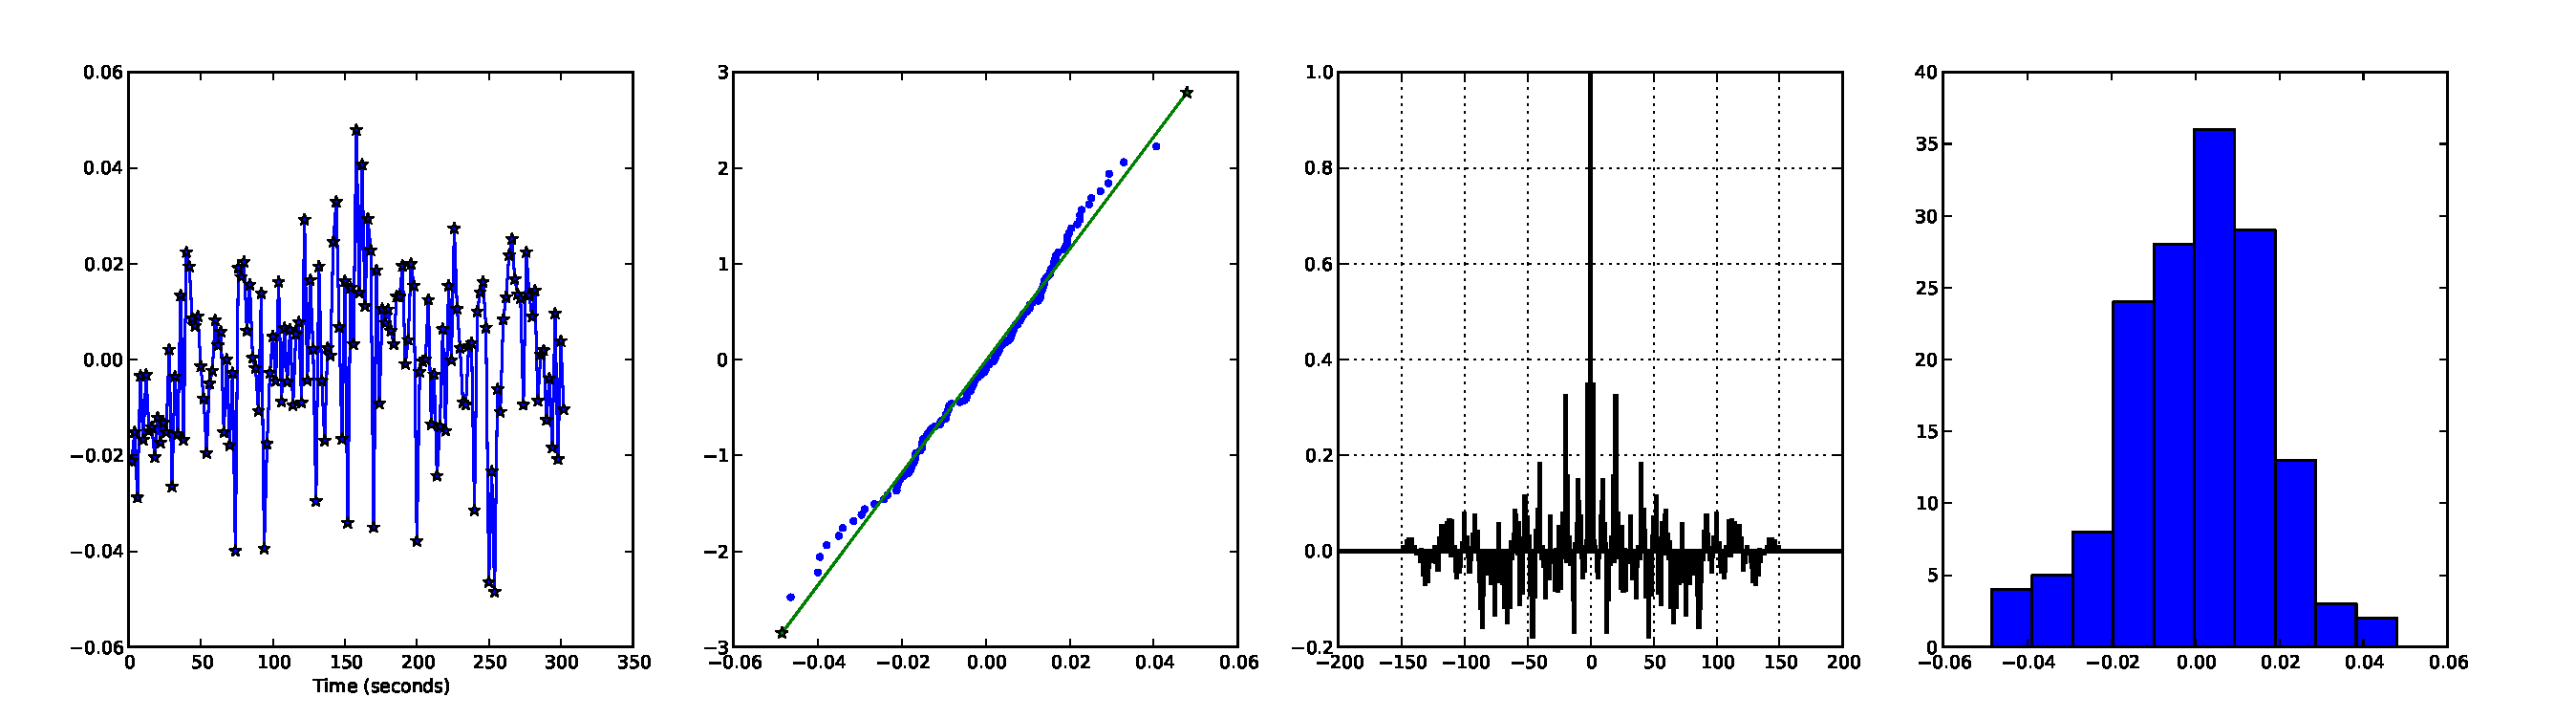
\includegraphics[trim=6cm 1cm 6cm 0cm,width=14cm]{images/noise2_0009_29_49_9}}
\subfigure[]{\label{fig:QQDC:B}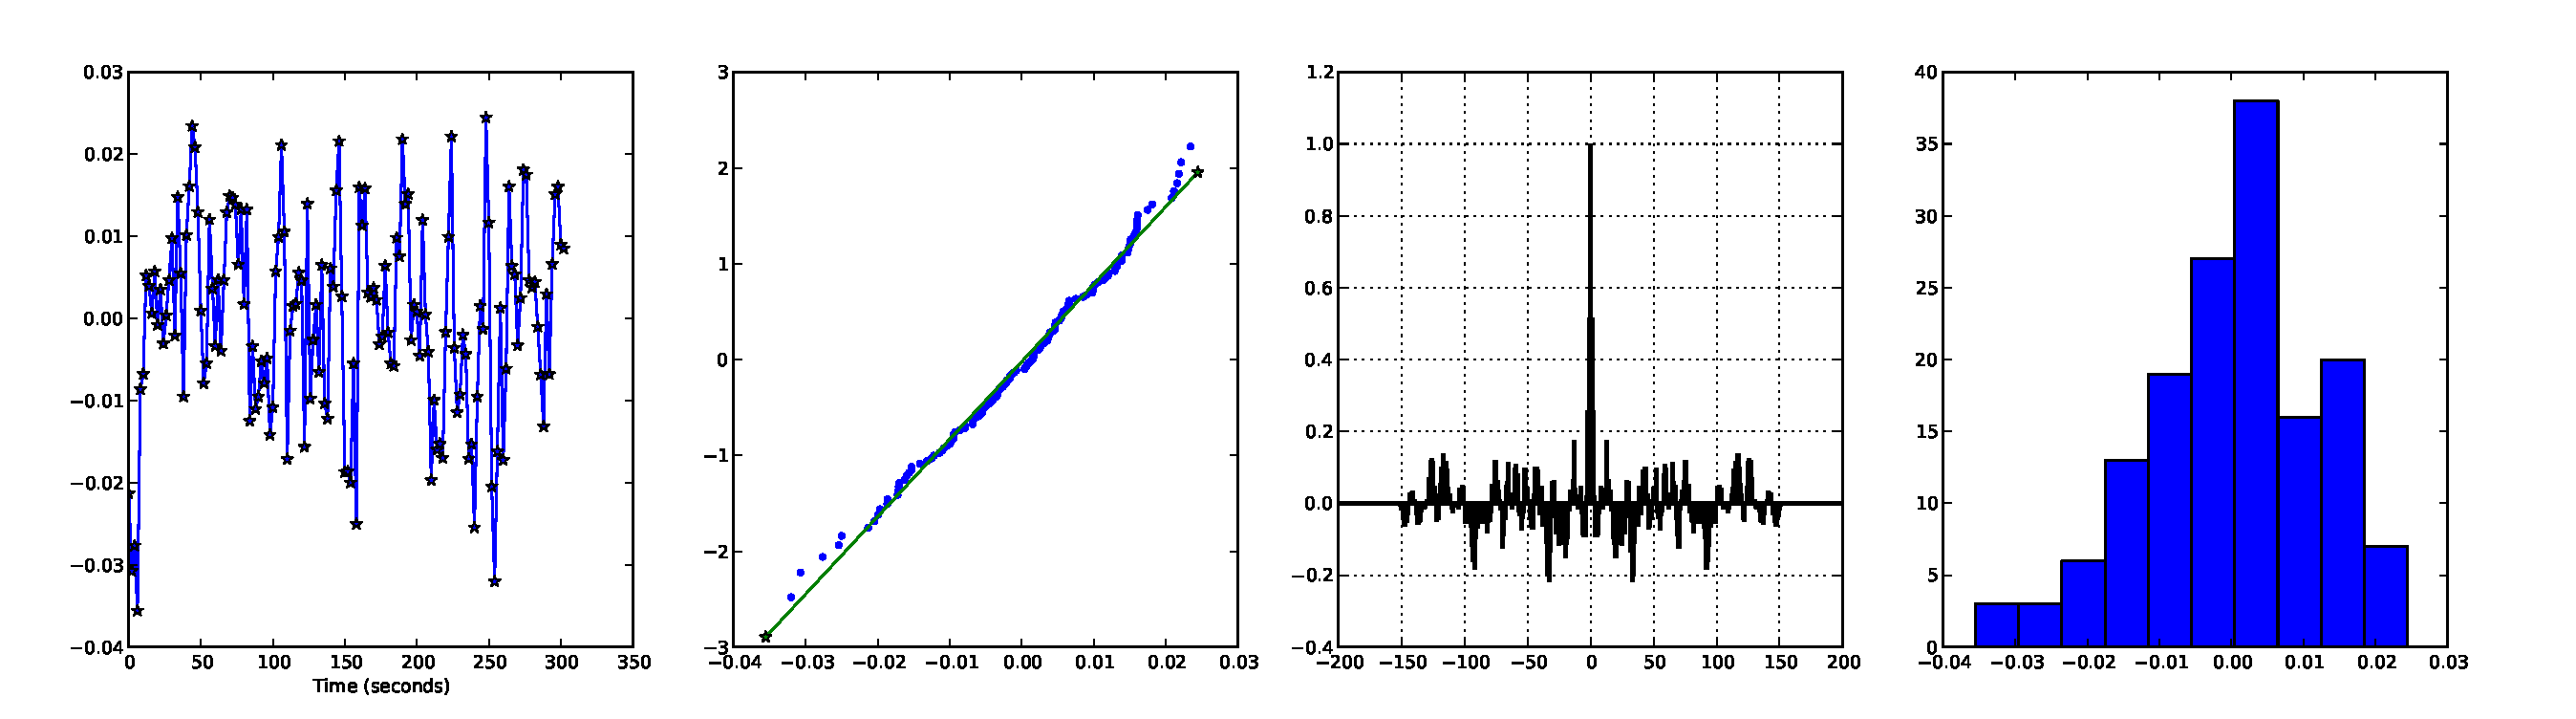
\includegraphics[trim=6cm 1cm 6cm 0cm,width=14cm]{images/noise2_0009_34_43_24}}
\subfigure[]{\label{fig:QQDC:C}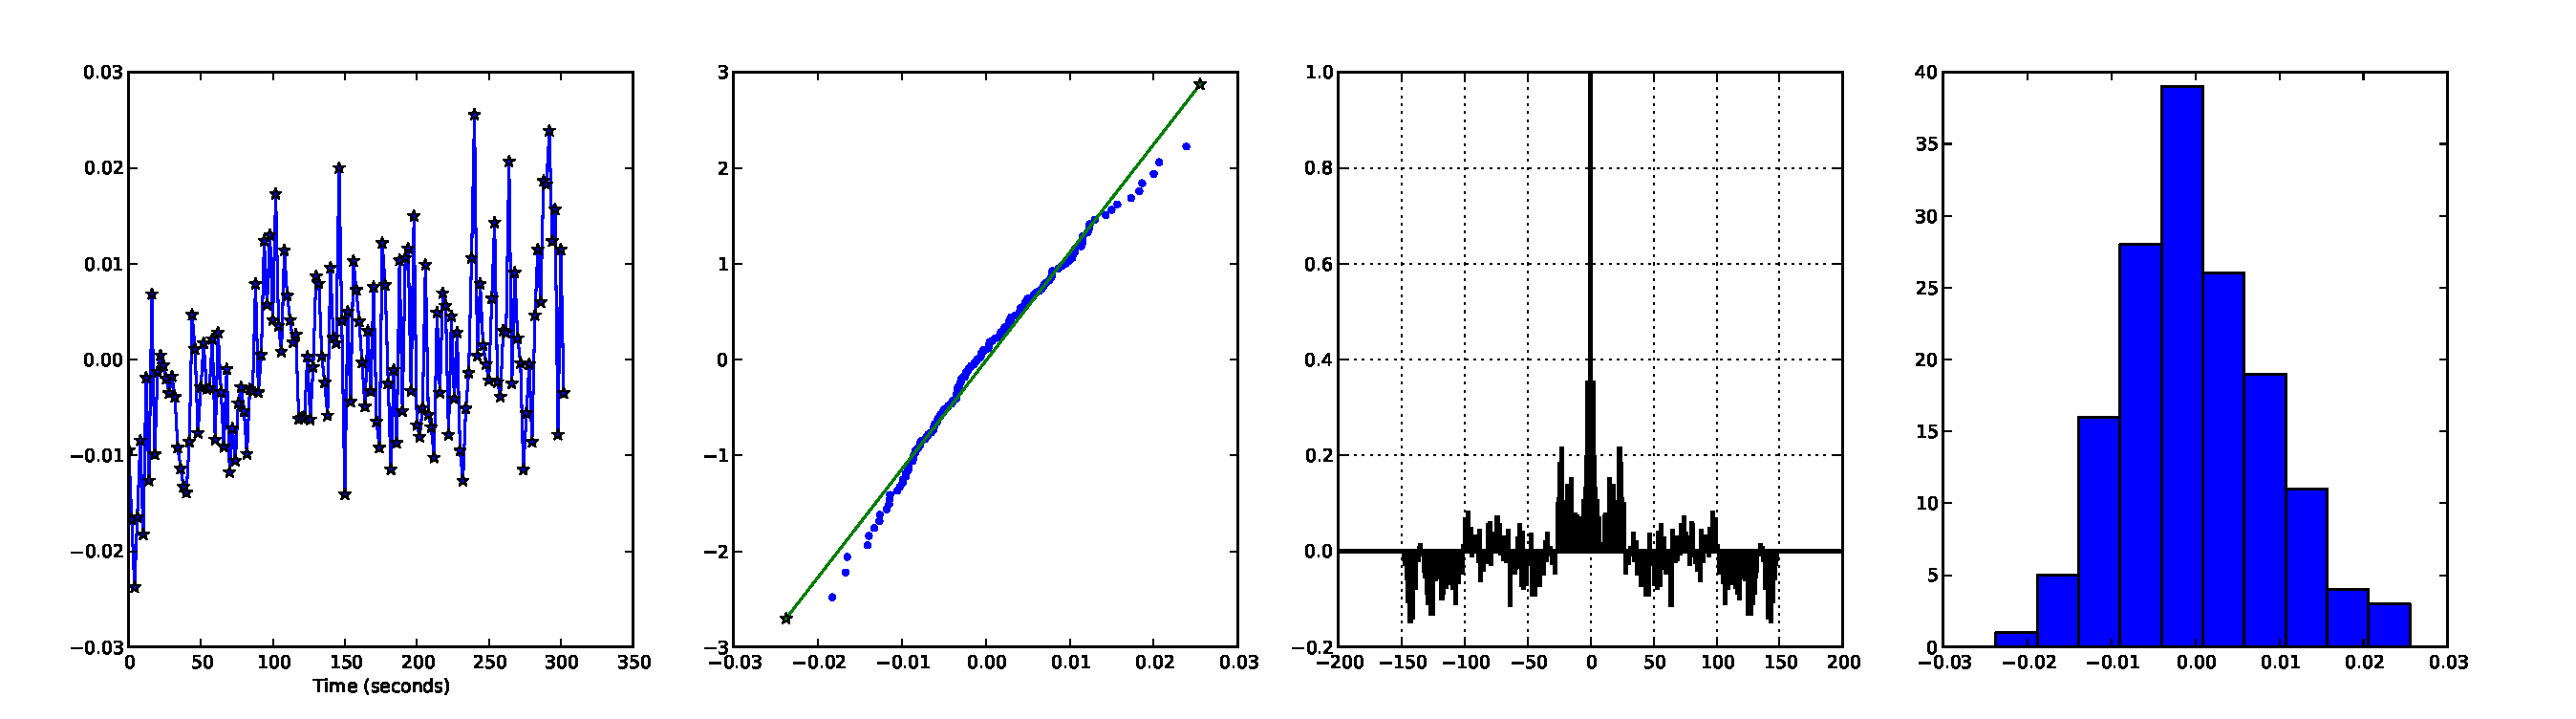
\includegraphics[trim=6cm 1cm 6cm 0cm,width=14cm]{images/noise2_0009_22_38_23}}
\subfigure[]{\label{fig:QQDC:D}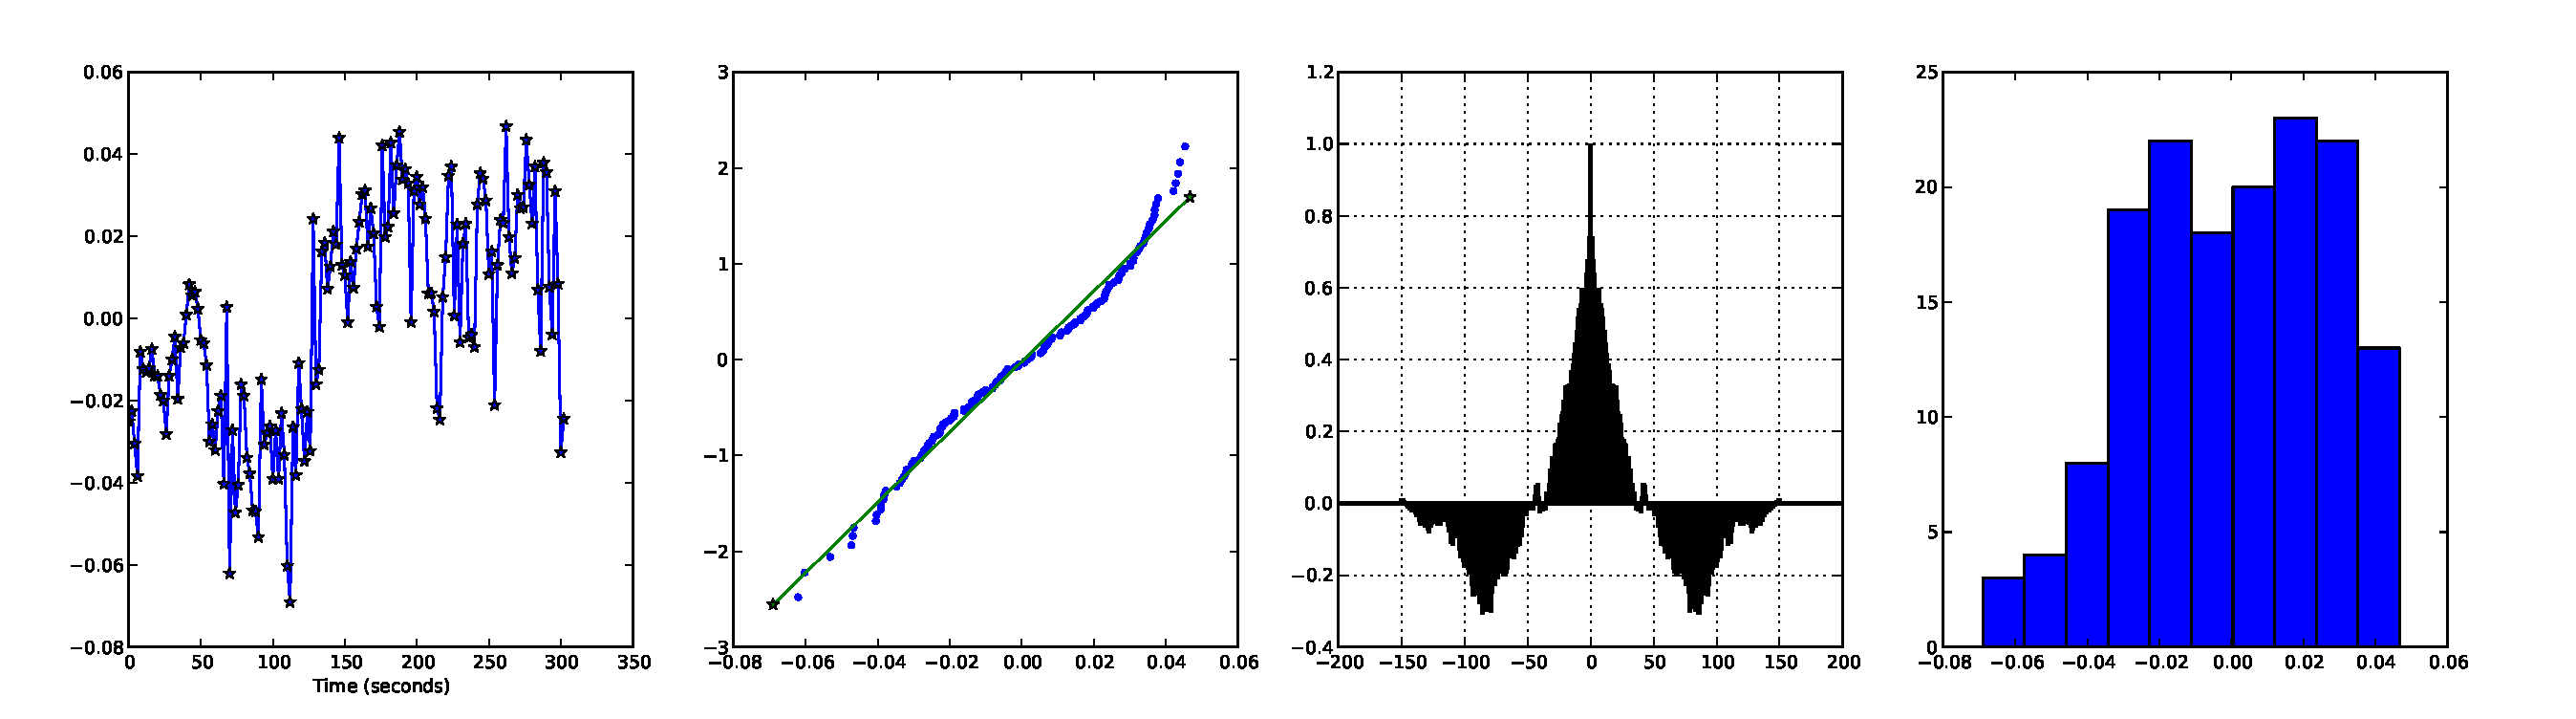
\includegraphics[trim=6cm 1cm 6cm 0cm,width=14cm]{images/noise2_0009_37_29_24}}

%\subfigure{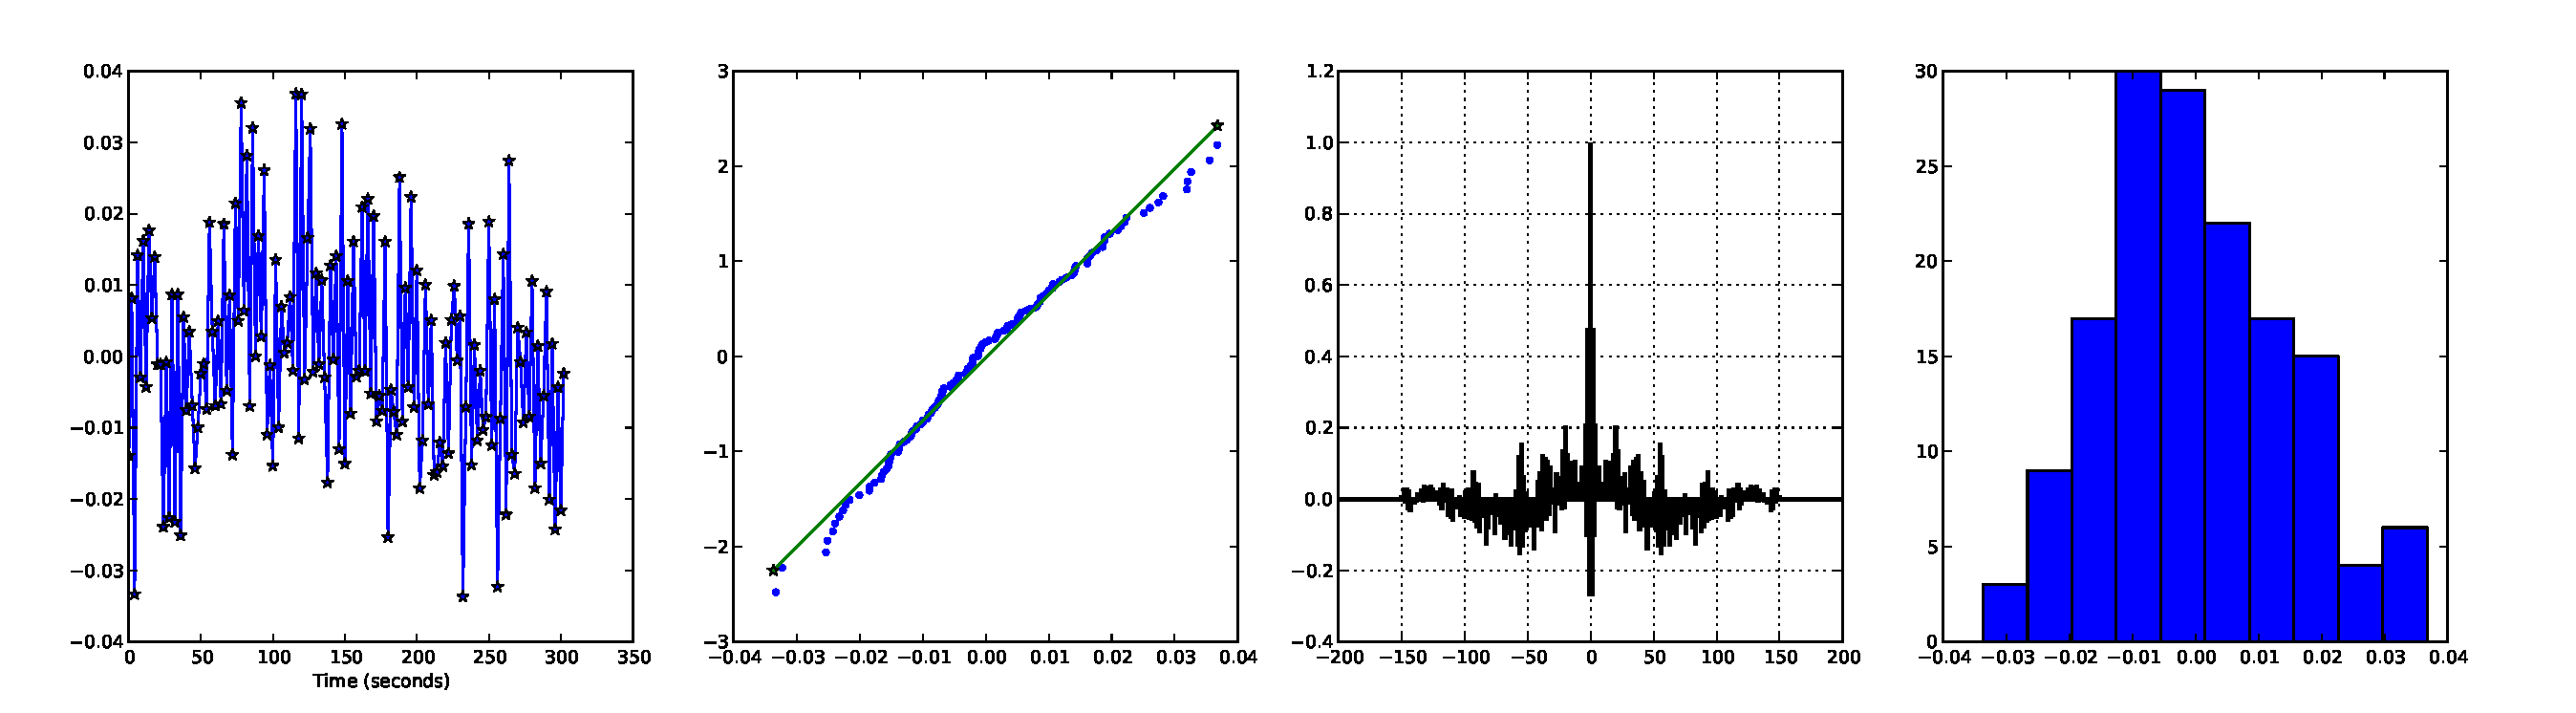
\includegraphics[trim=6cm 1cm 0 0cm,width=17cm]{images/noise_0009_19-24-10.pdf}}
%\subfigure{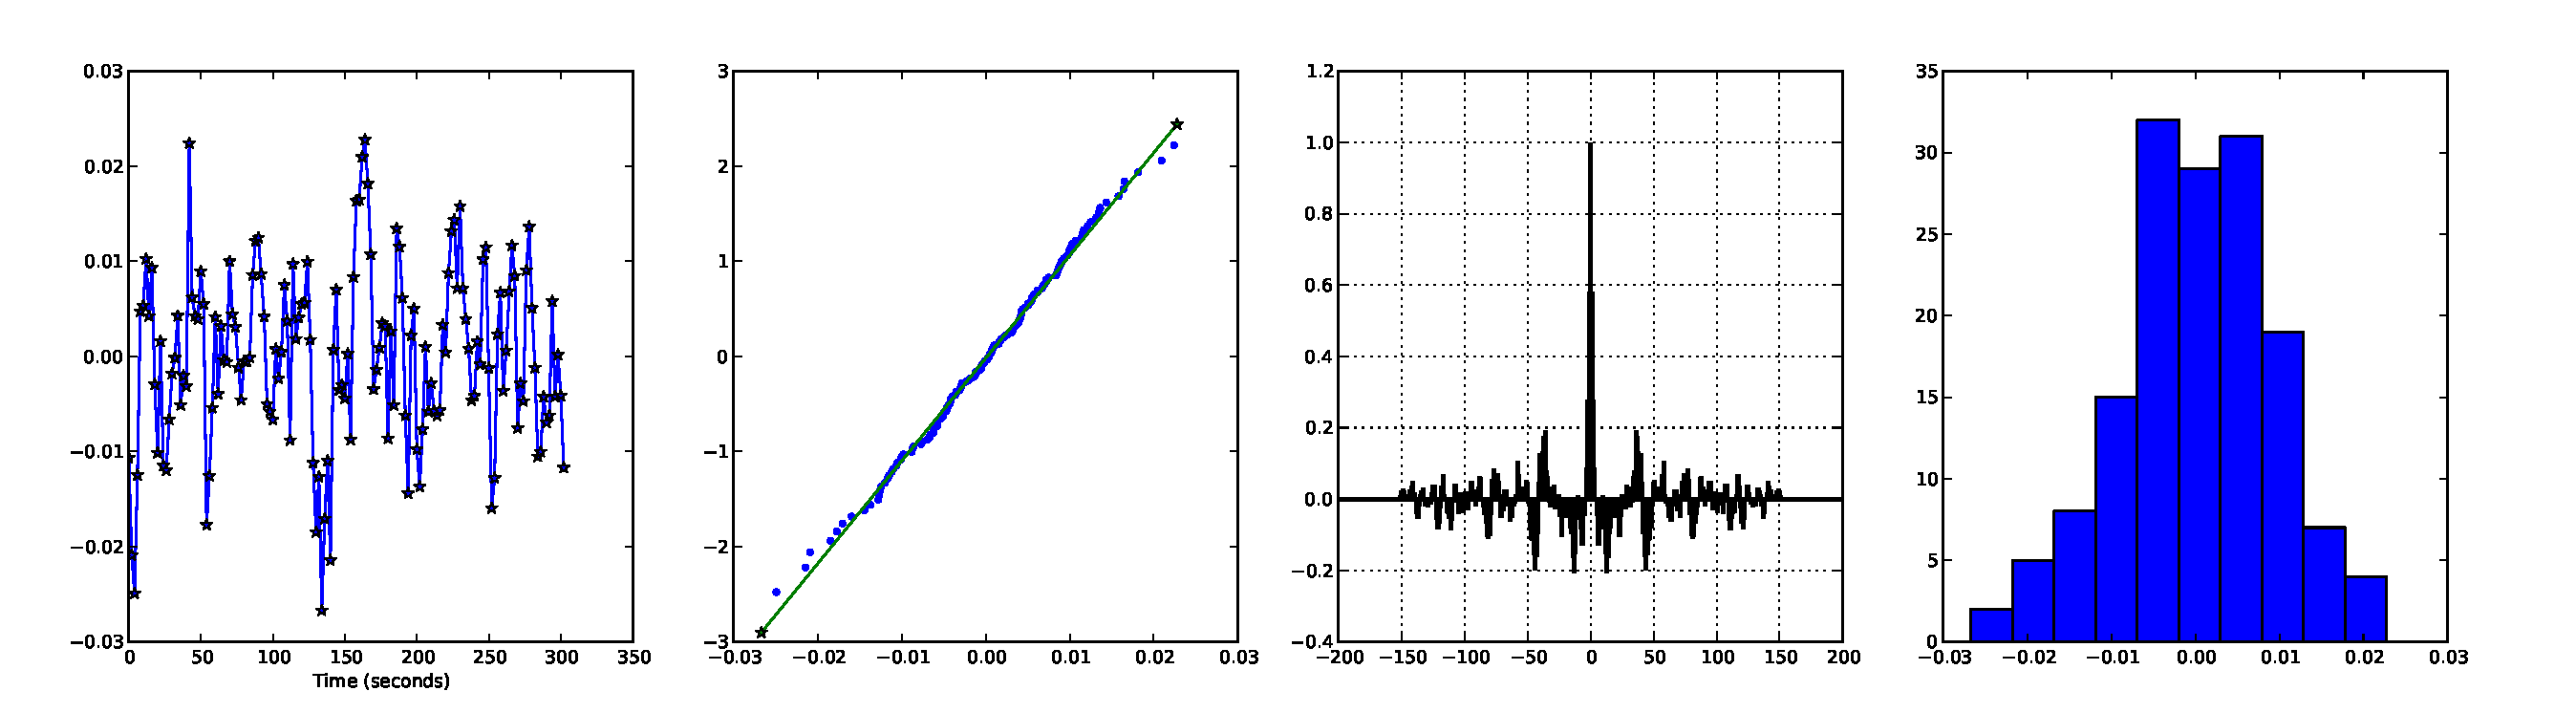
\includegraphics[trim=6cm 1cm 0 0cm,width=17cm]{images/noise_0009_20-45-18.pdf}}
%\subfigure{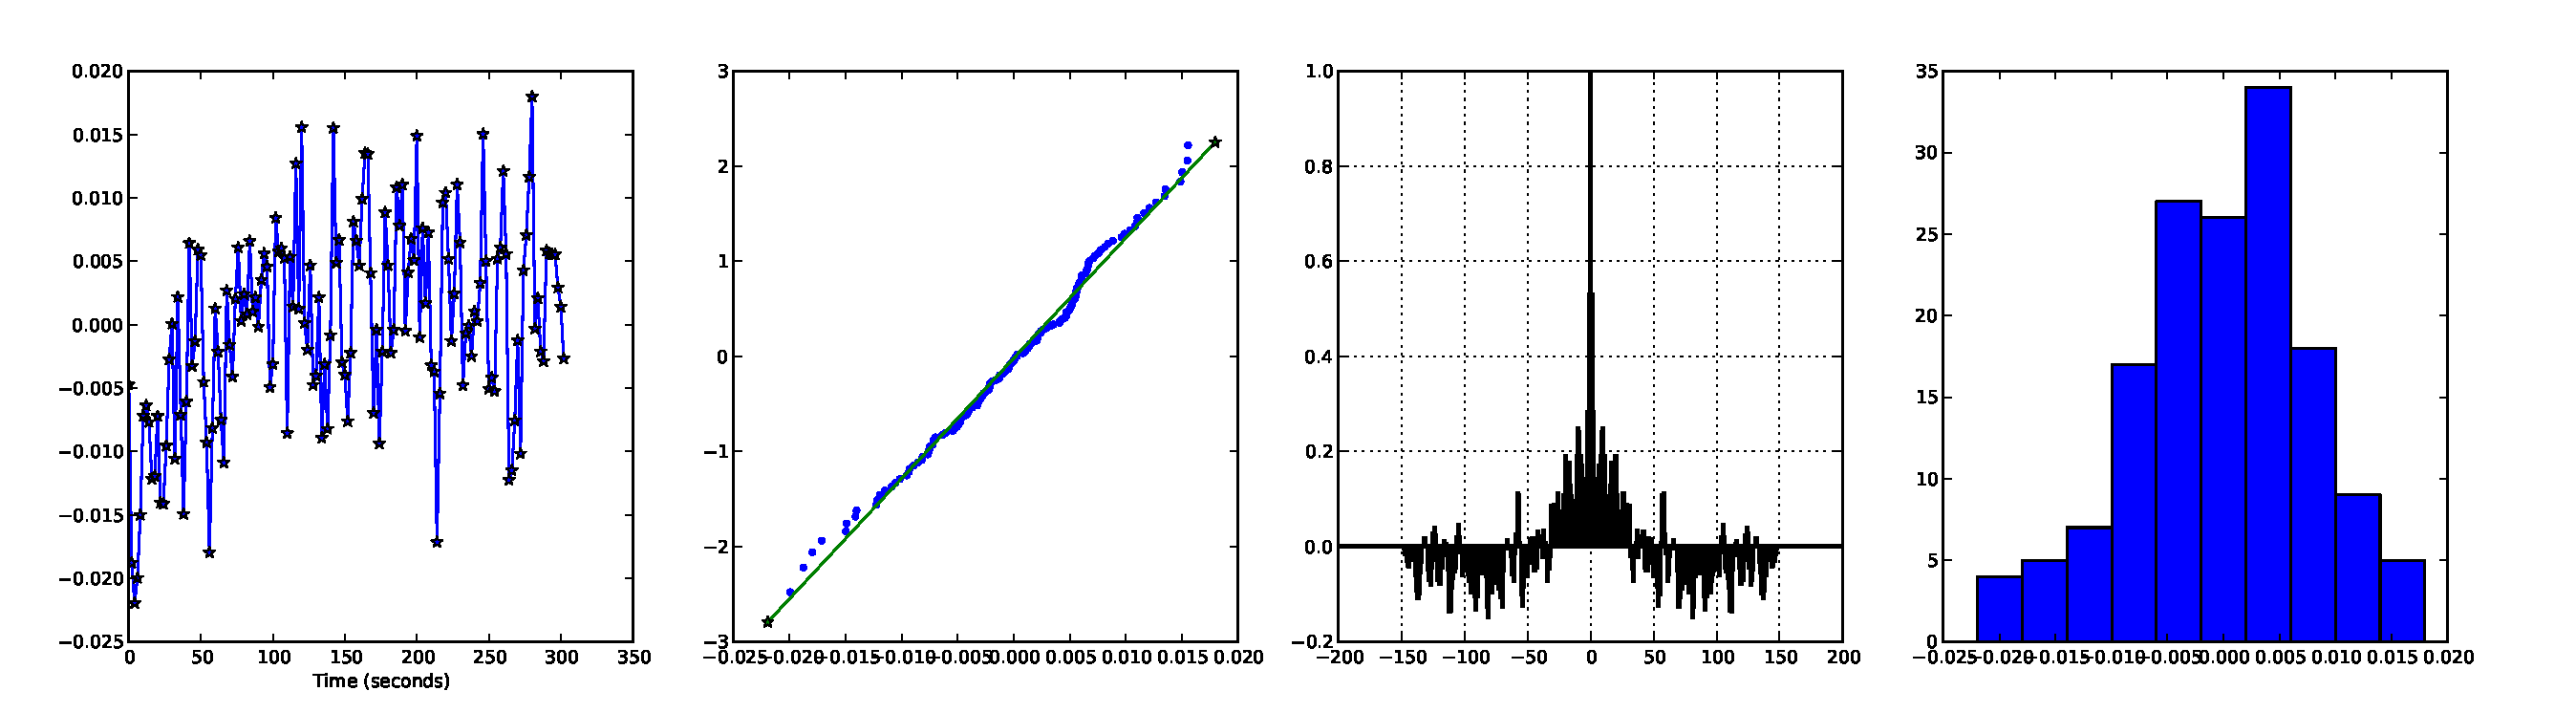
\includegraphics[trim=6cm 1cm 0 0cm,width=17cm]{images/noise_0009_23-47-18.pdf}}
%\subfigure{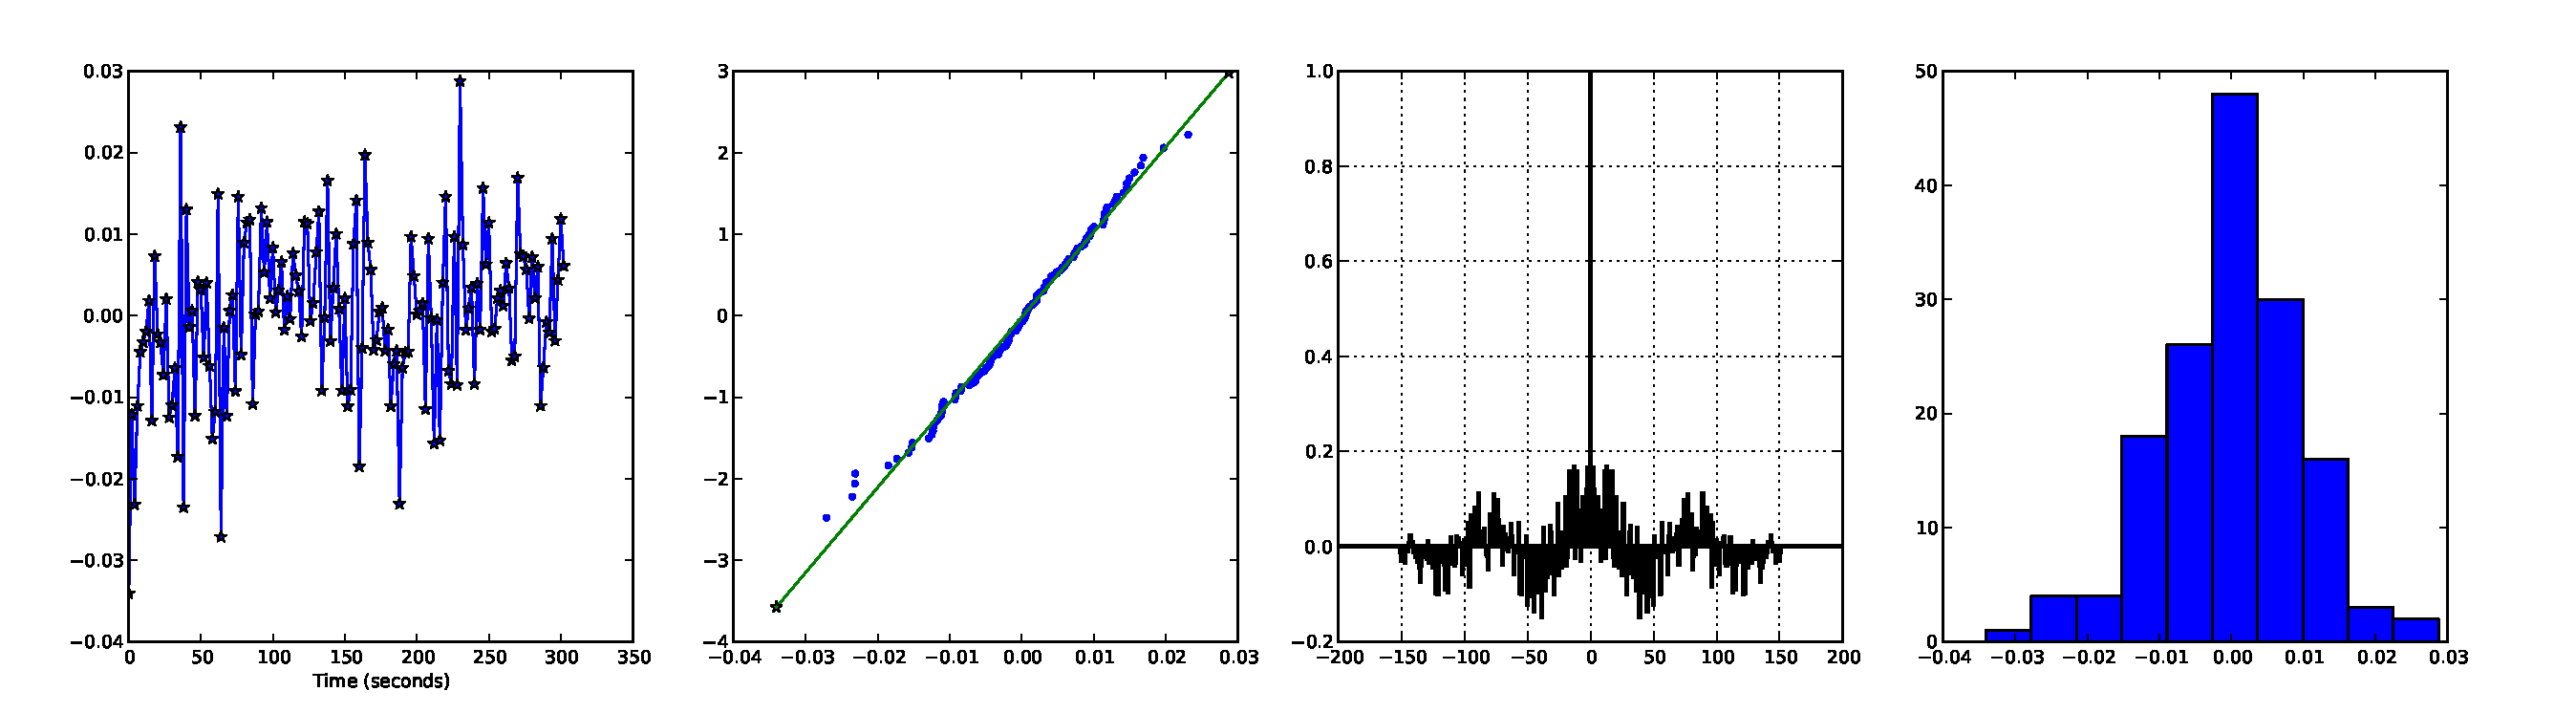
\includegraphics[trim=6cm 1cm 0 0cm,width=17cm]{images/noise_0009_35-49-9.pdf}}

\caption{Q-Q Plots of normalized resting state data}
\label{fig:QQDC}
\end{figure}

\begin{figure}
\centering
\subfigure[]{\label{fig:QQDDlta:A}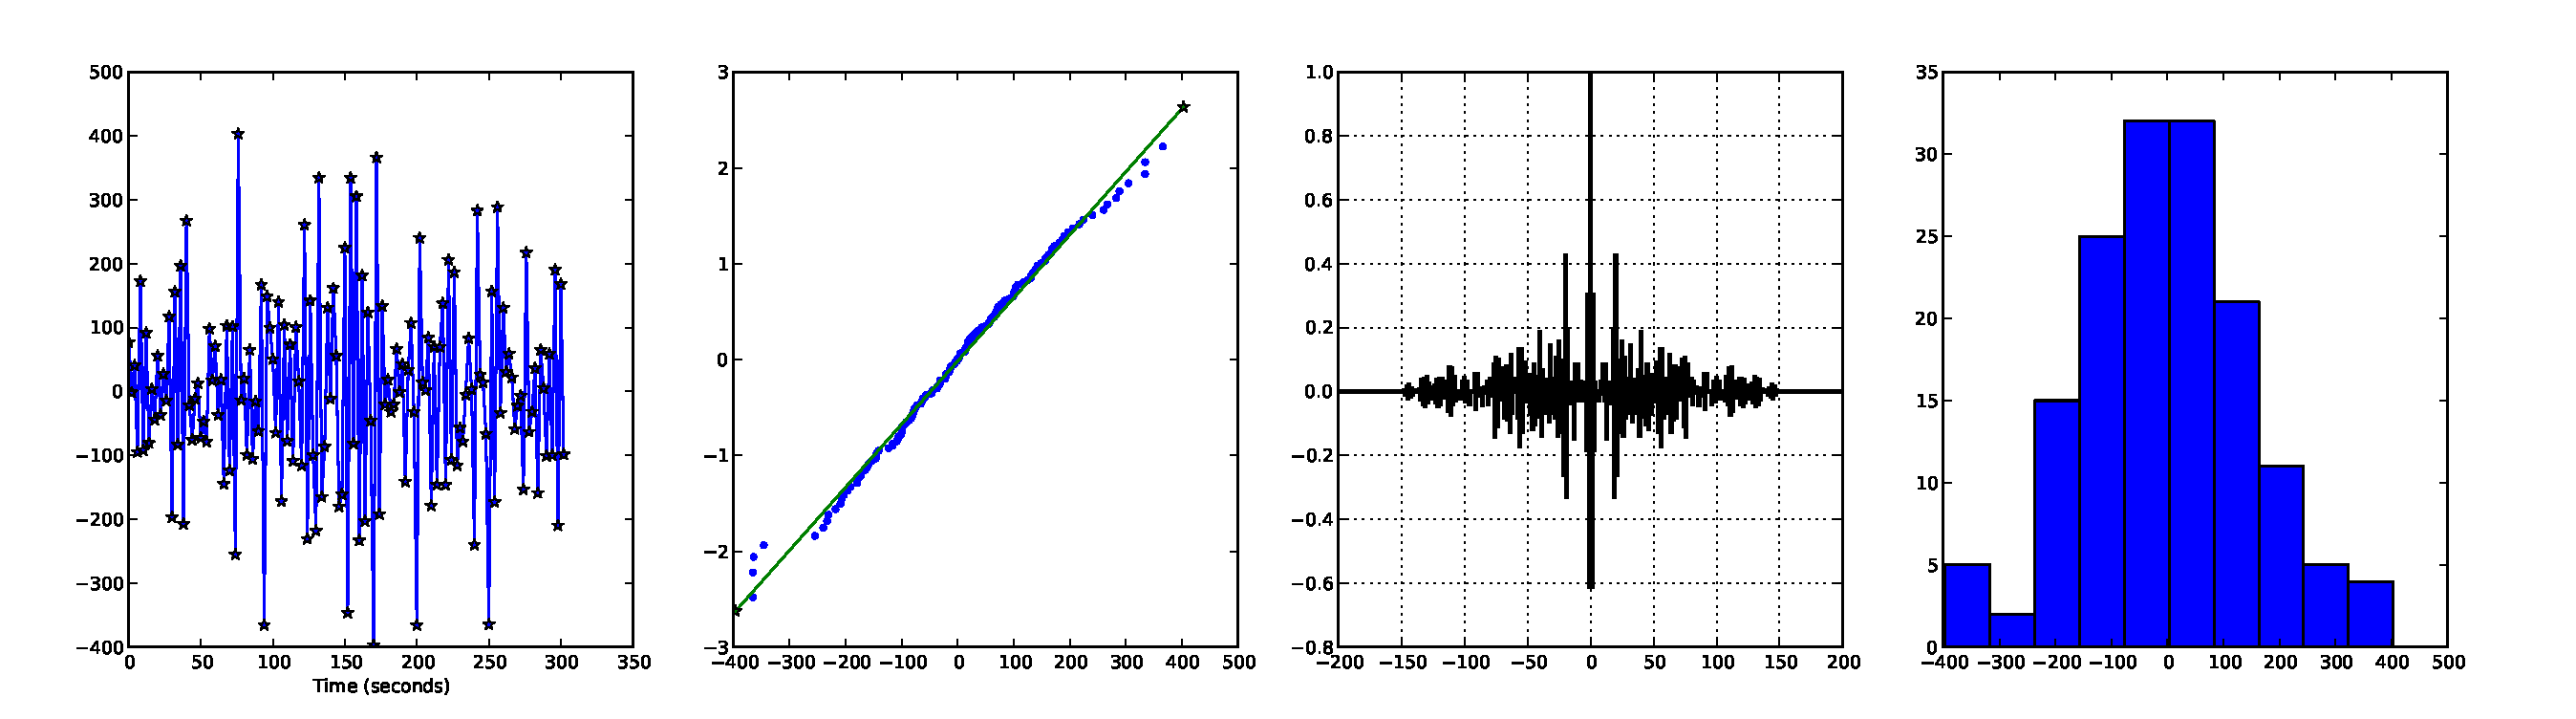
\includegraphics[trim=6cm 1cm 6cm 0,width=14cm]{images/noise2_0009d_29_49_9}}
\subfigure[]{\label{fig:QQDDlta:B}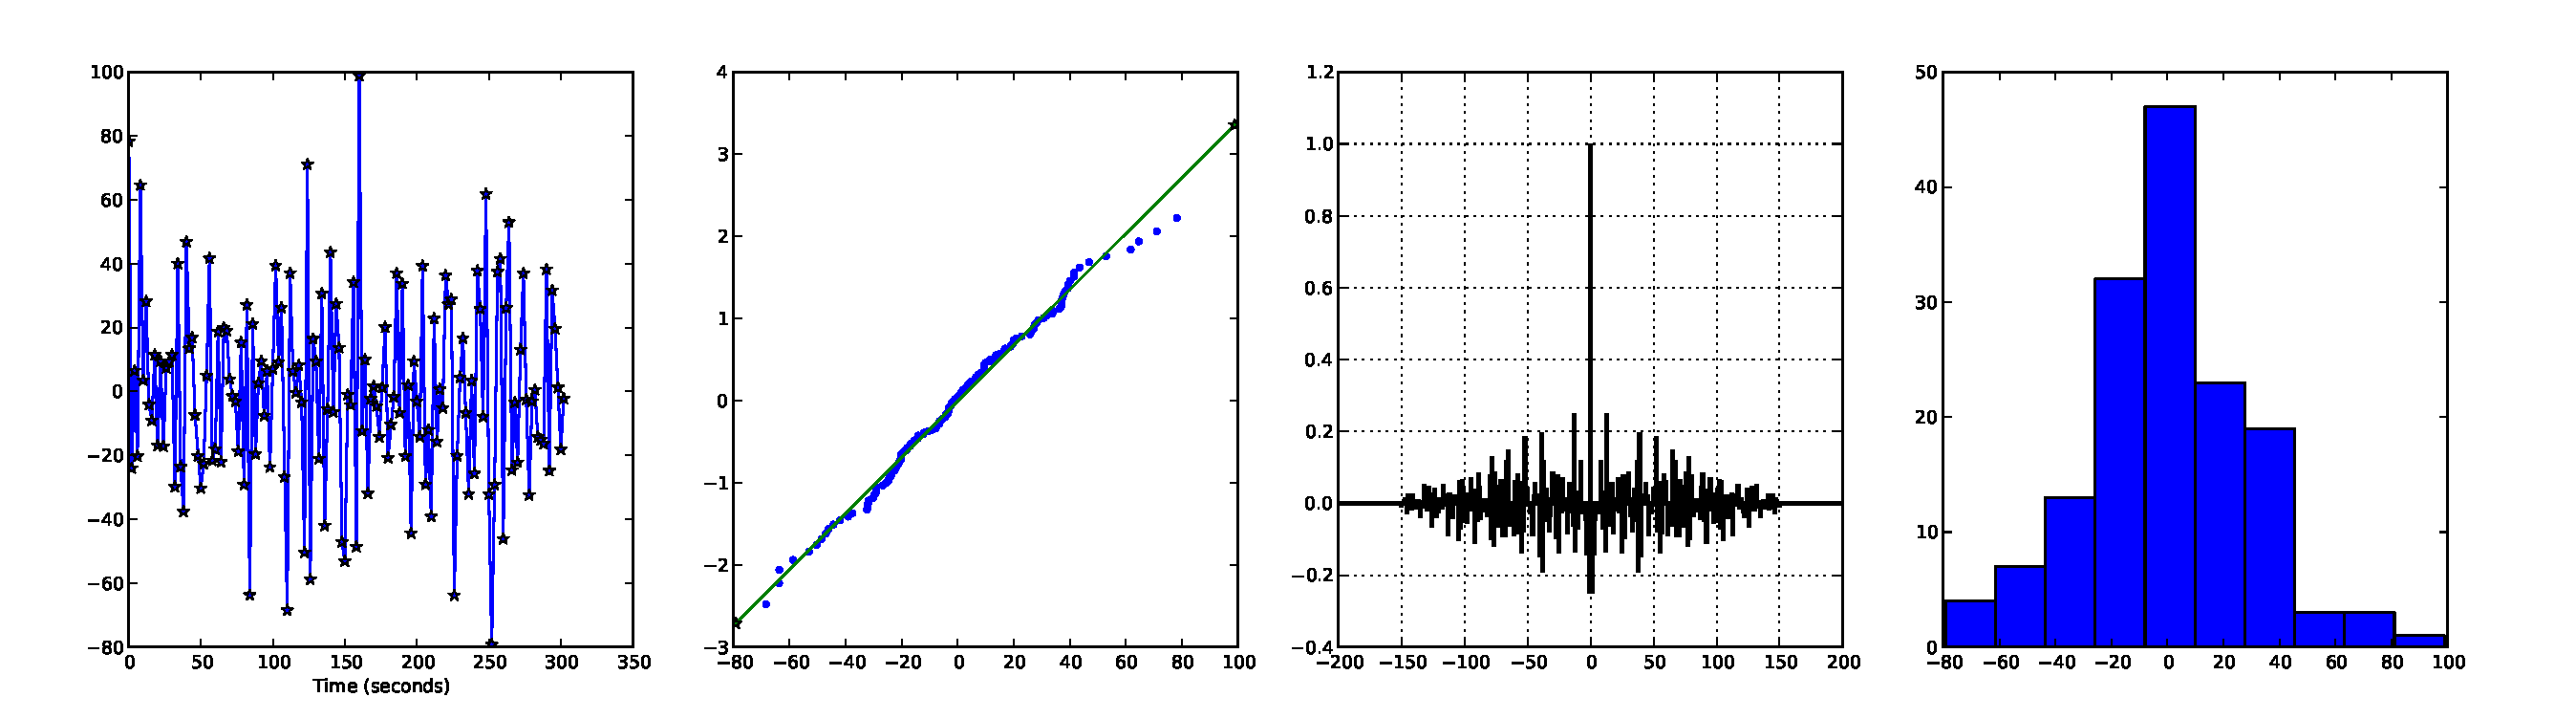
\includegraphics[trim=6cm 1cm 6cm 0,width=14cm]{images/noise2_0009d_34_43_24}}
\subfigure[]{\label{fig:QQDelta:C}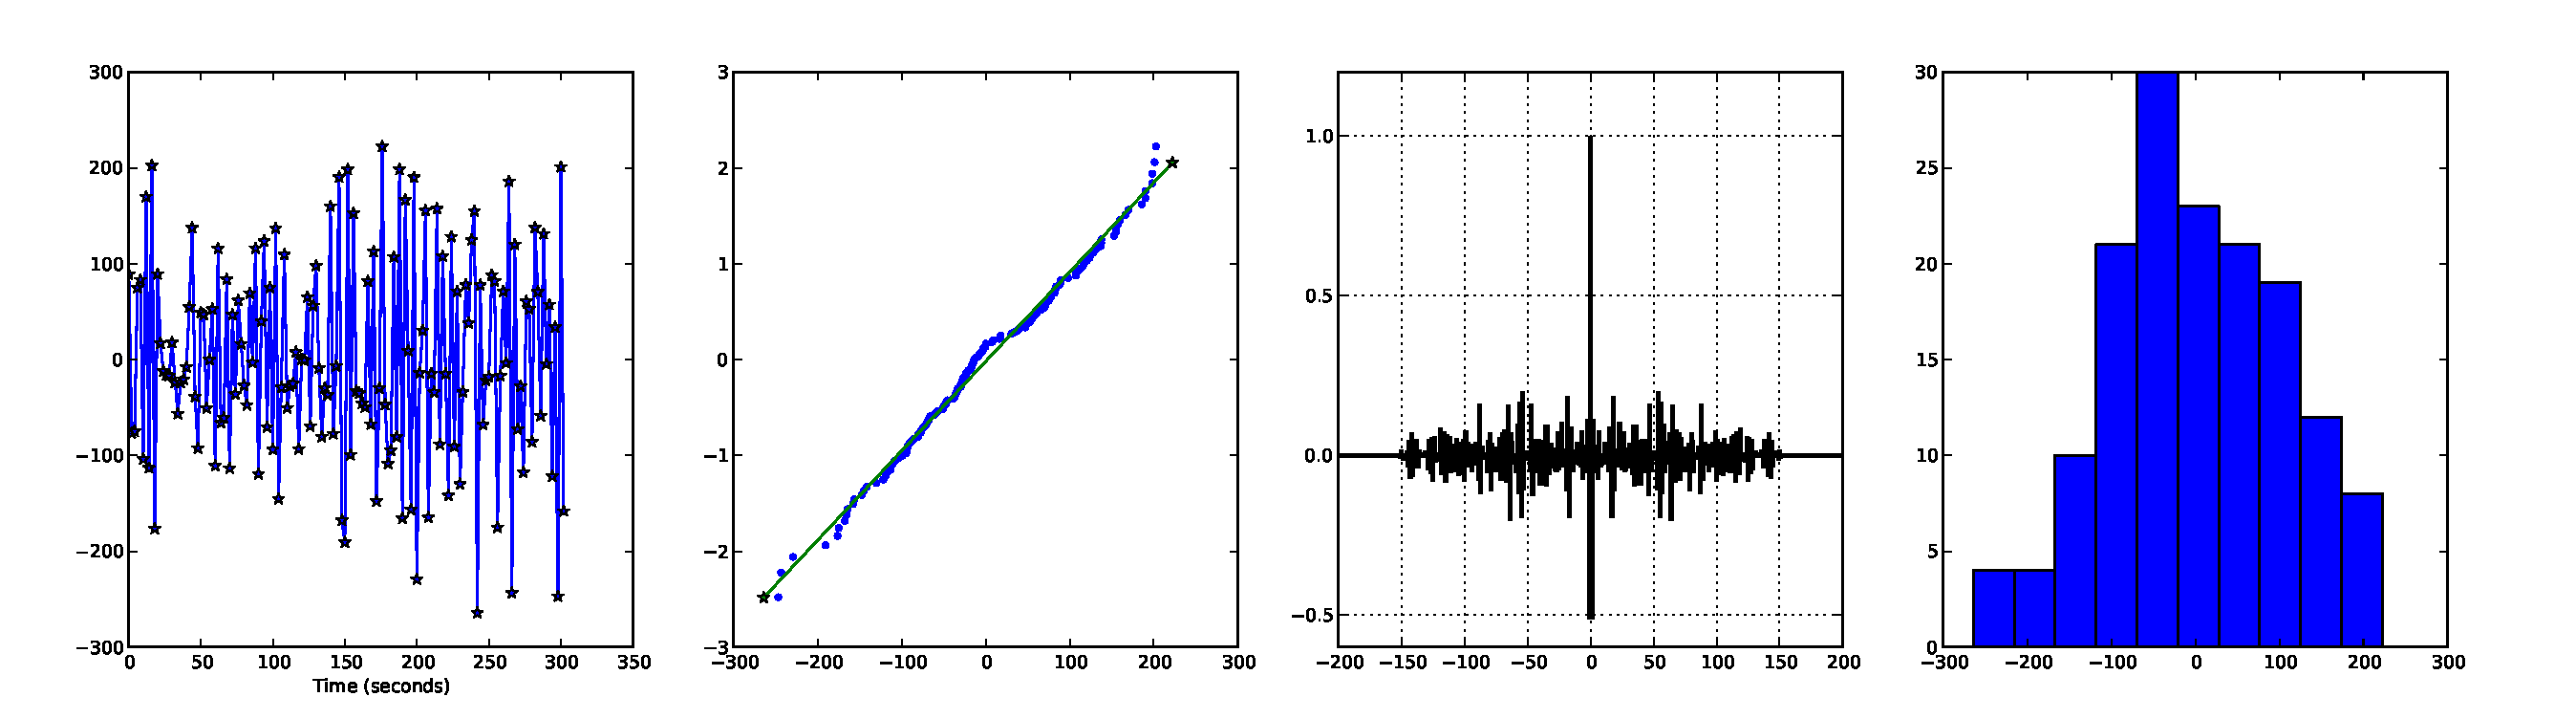
\includegraphics[trim=6cm 1cm 6cm 0,width=14cm]{images/noise2_0009d_22_38_23}}
\subfigure[]{\label{fig:QQDDlta:D}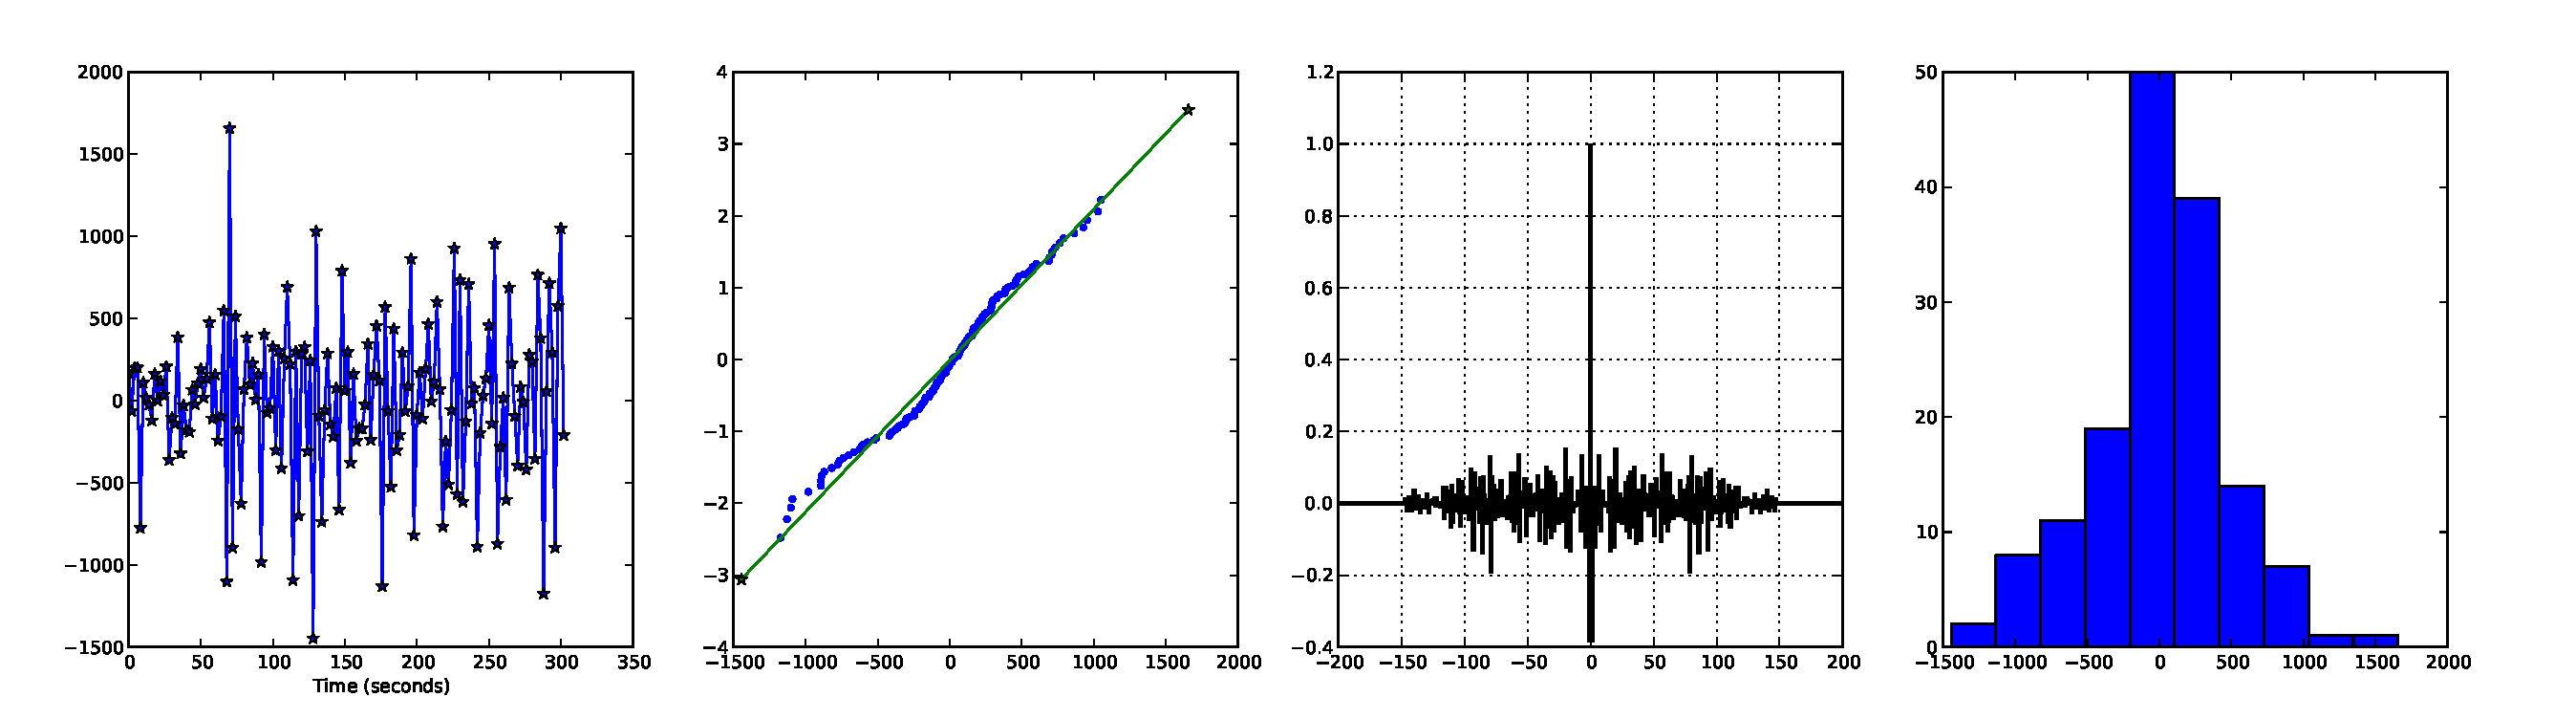
\includegraphics[trim=6cm 1cm 6cm 0,width=14cm]{images/noise2_0009d_37_29_24}}
\caption{Q-Q Plots of resting state data, using the BOLD signal changes}
\label{fig:QQDelta}
\end{figure}

A Wiener process should still conform to the normal distribution, with a 
variance proportional to the run-time. Note that \autoref{fig:QQDC:A} and \autoref{fig:QQDC:B}
are relatively well described by a Gaussian process with a small autocorrelation, 
\autoref{fig:QQDC:C} and \autoref{fig:QQDC:D} are not. In particular the tails of \autoref{fig:QQDC:C}
do not seem to fit the Gaussian well. Also note the significant autocorrelation in
\autoref{fig:QQDC:C} and \autoref{fig:QQDC:D}. As expected, the noise is not strictly
Gaussian white noise.  On the other hand, the steps do conform rather
closely to the normal distribution.
As expected, most of the autocorrelation disappears for the step data. Given
that the steps seem to fit the Normal distribution, the low autocorrelation
indicates that the steps could be Independently Distributed. 
Therefore, the assumption that the noise follows a Wiener process seems to
be correct. 

\begin{figure}
\centering
\subfigure[]{\label{fig:QQs:A}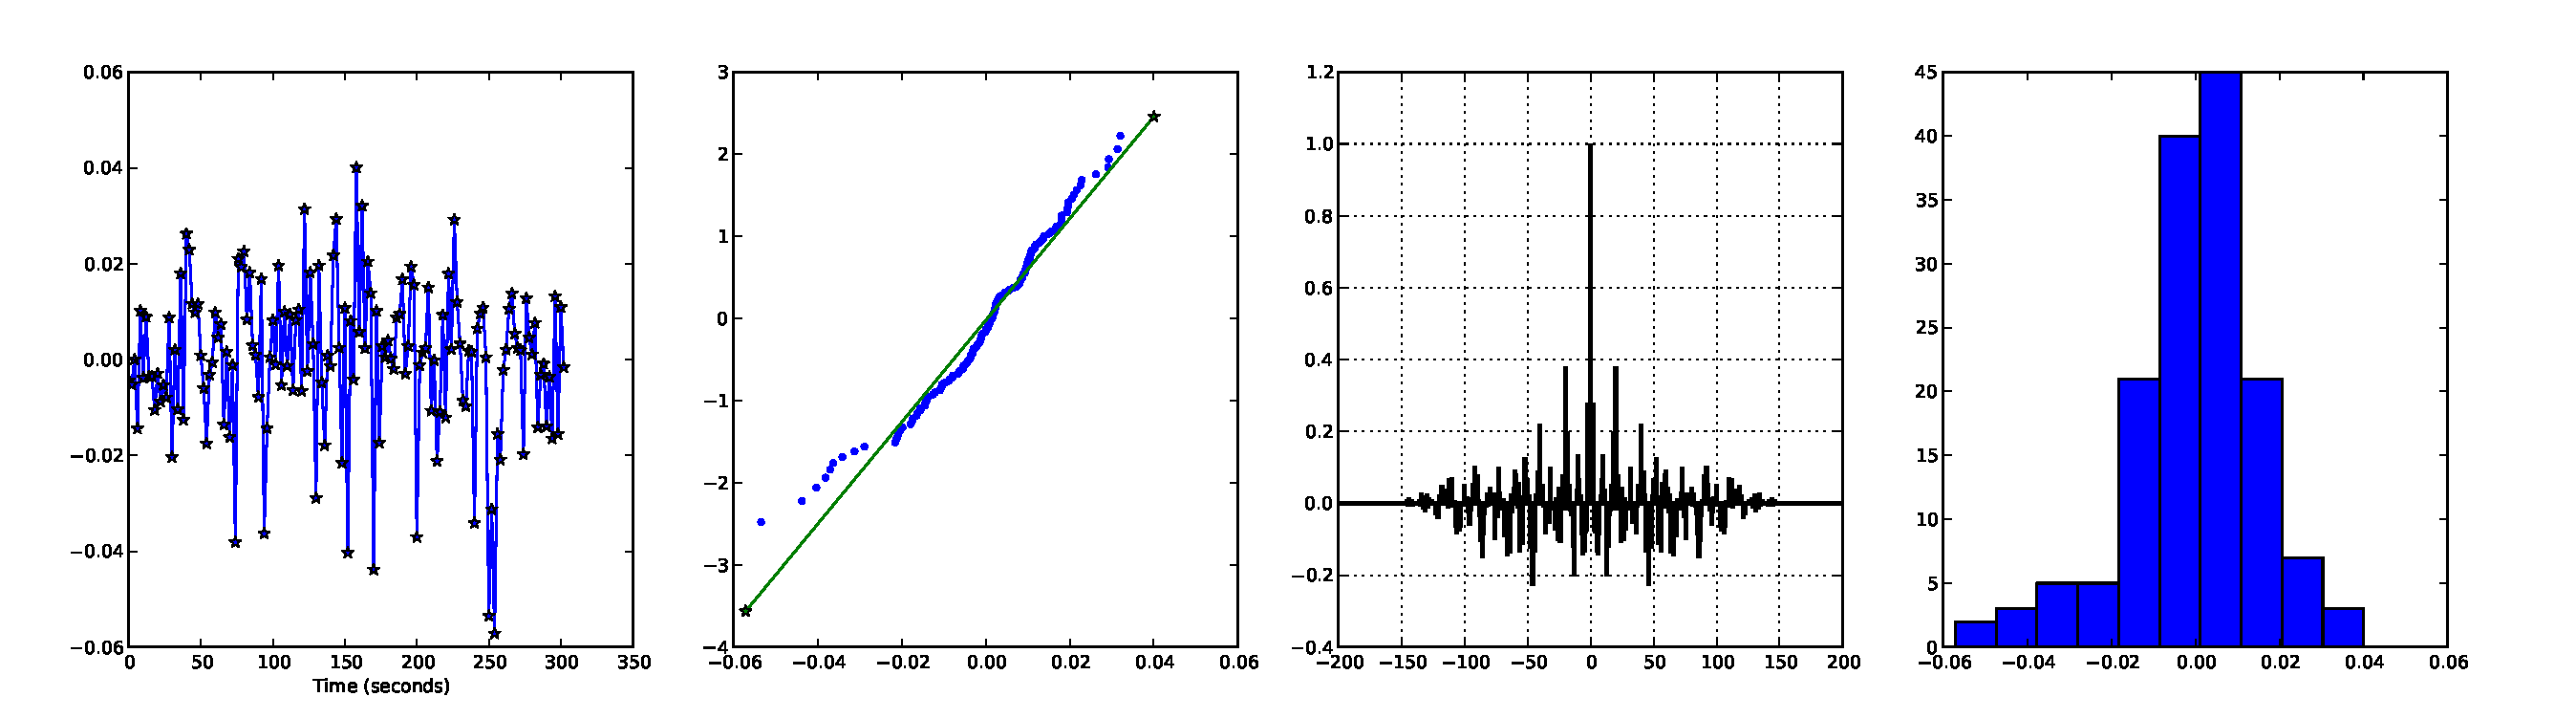
\includegraphics[trim=6cm 1cm 6cm 0cm,width=14cm]{images/noise2_0009s_29_49_9}}
\subfigure[]{\label{fig:QQs:B}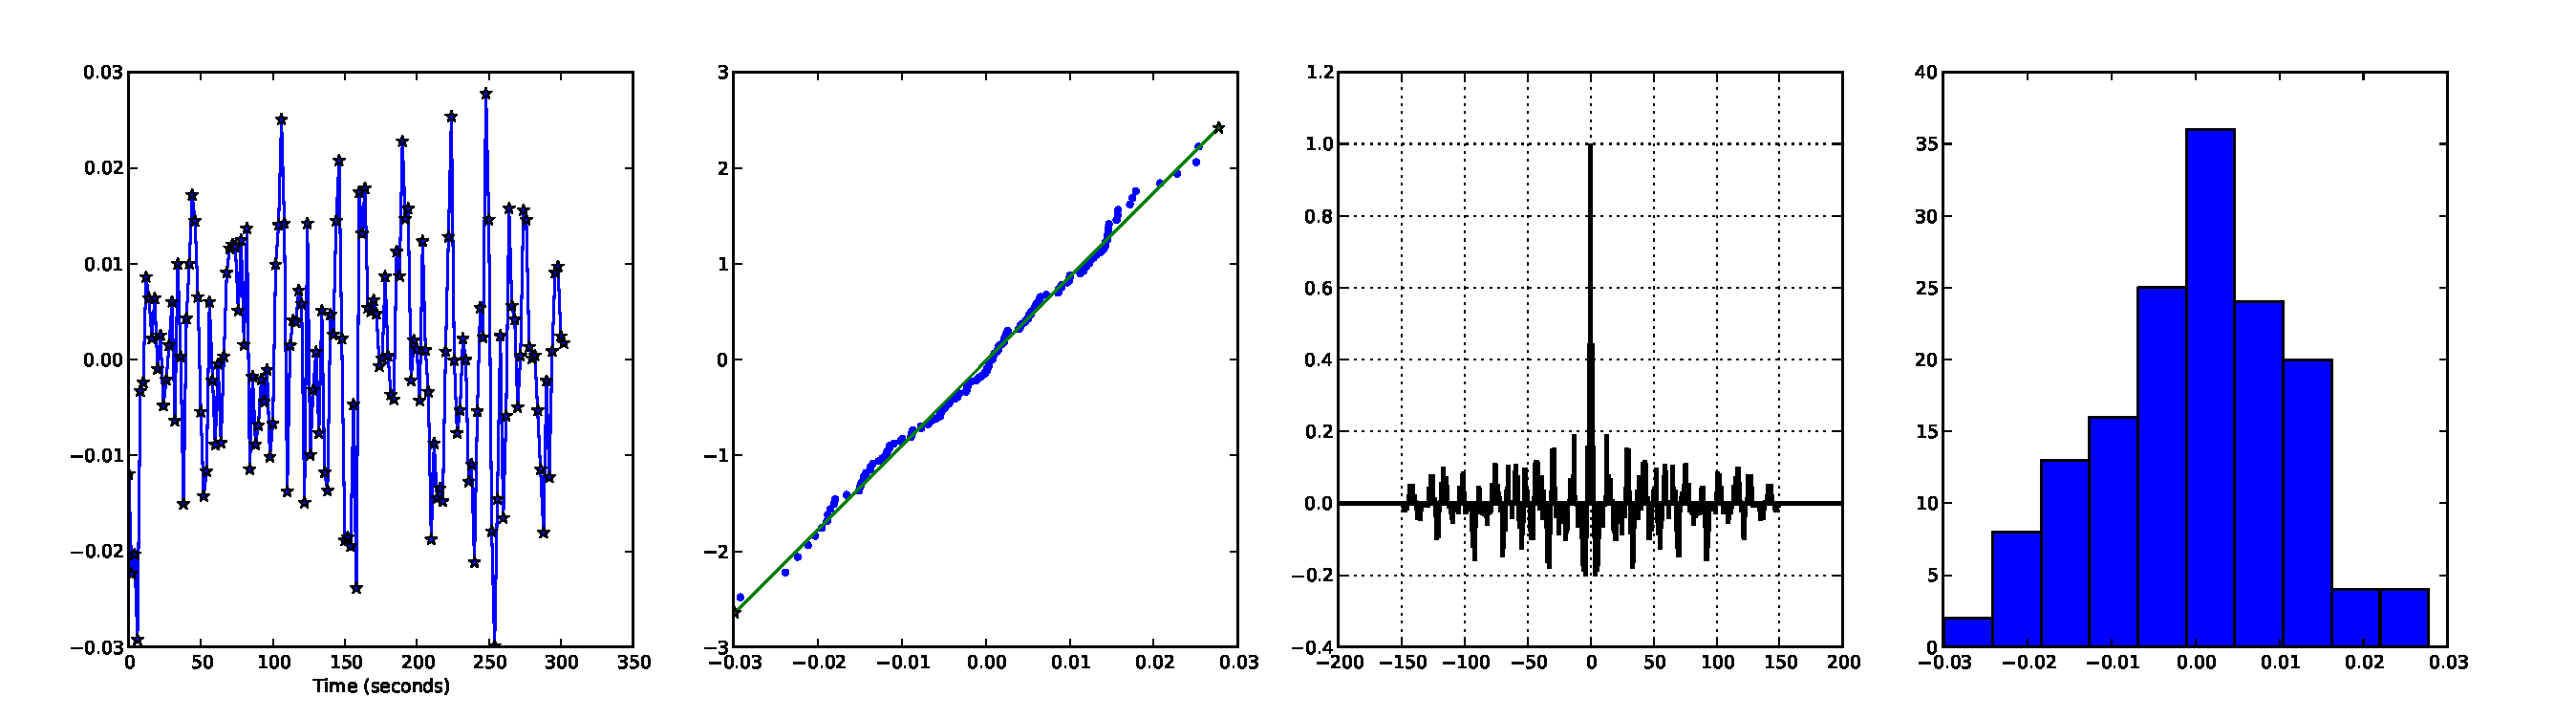
\includegraphics[trim=6cm 1cm 6cm 0cm,width=14cm]{images/noise2_0009s_34_43_24}}
\subfigure[]{\label{fig:QQs:C}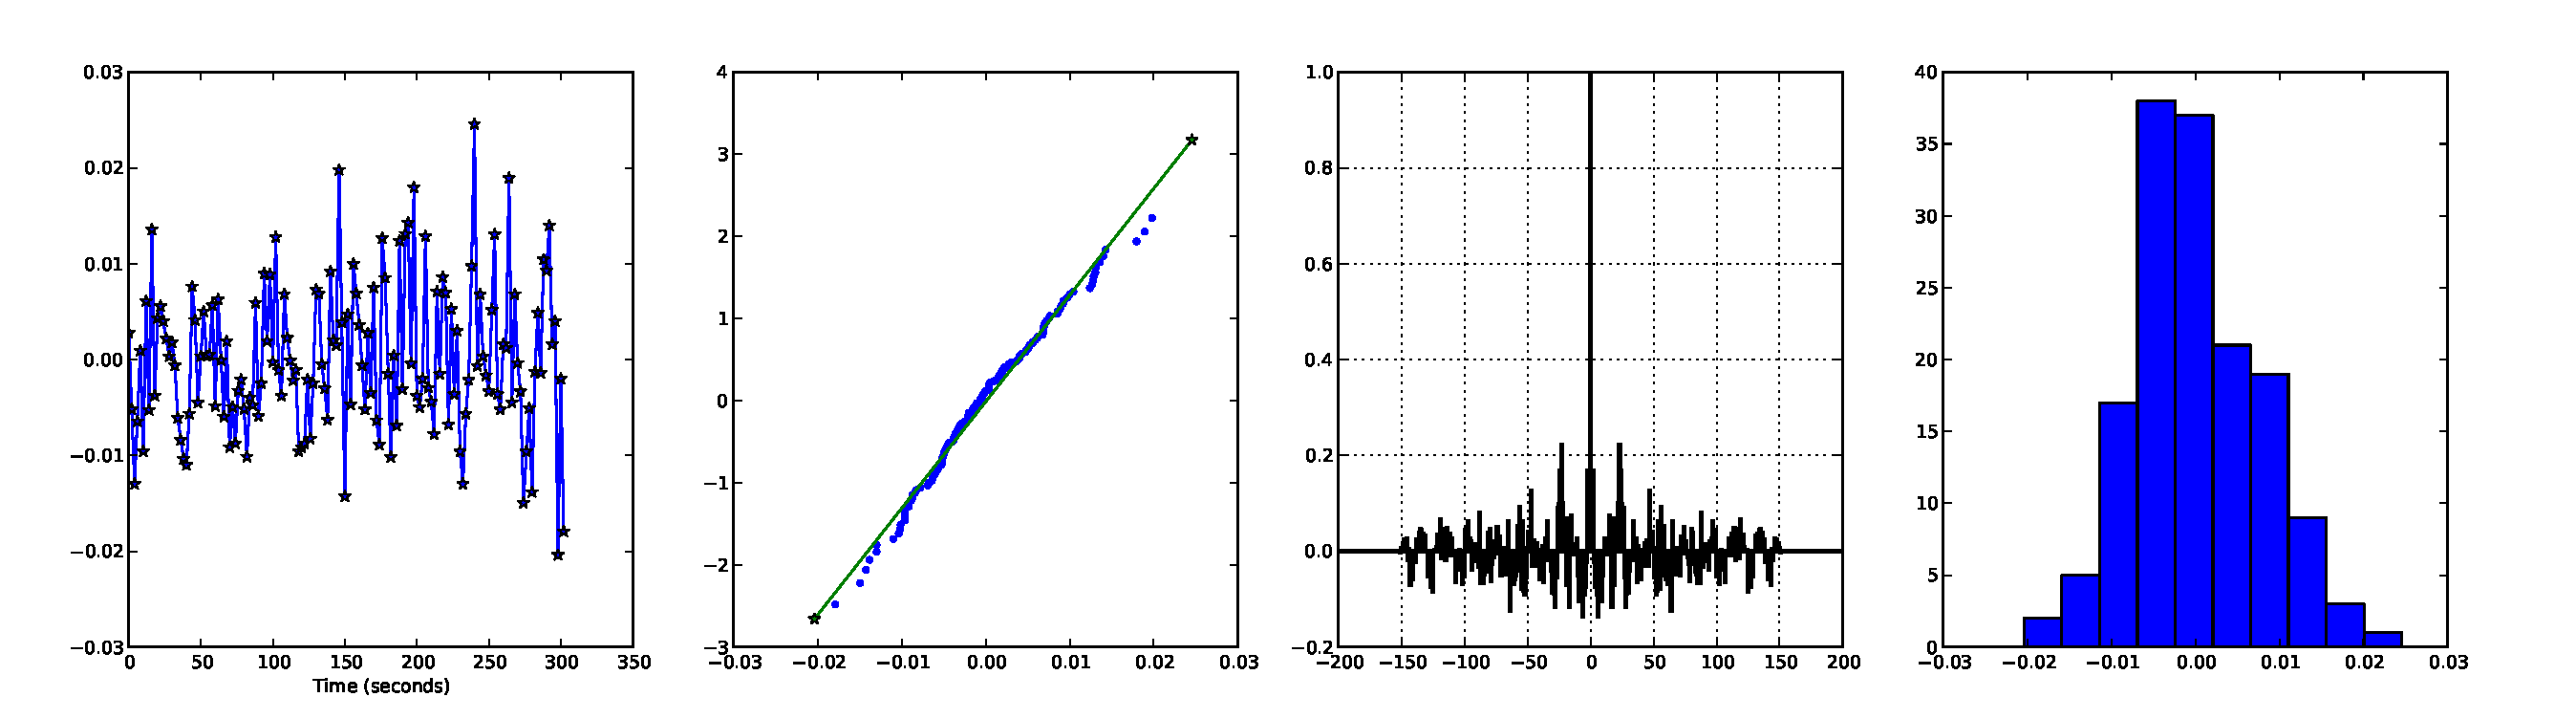
\includegraphics[trim=6cm 1cm 6cm 0cm,width=14cm]{images/noise2_0009s_22_38_23}}
\subfigure[]{\label{fig:QQs:D}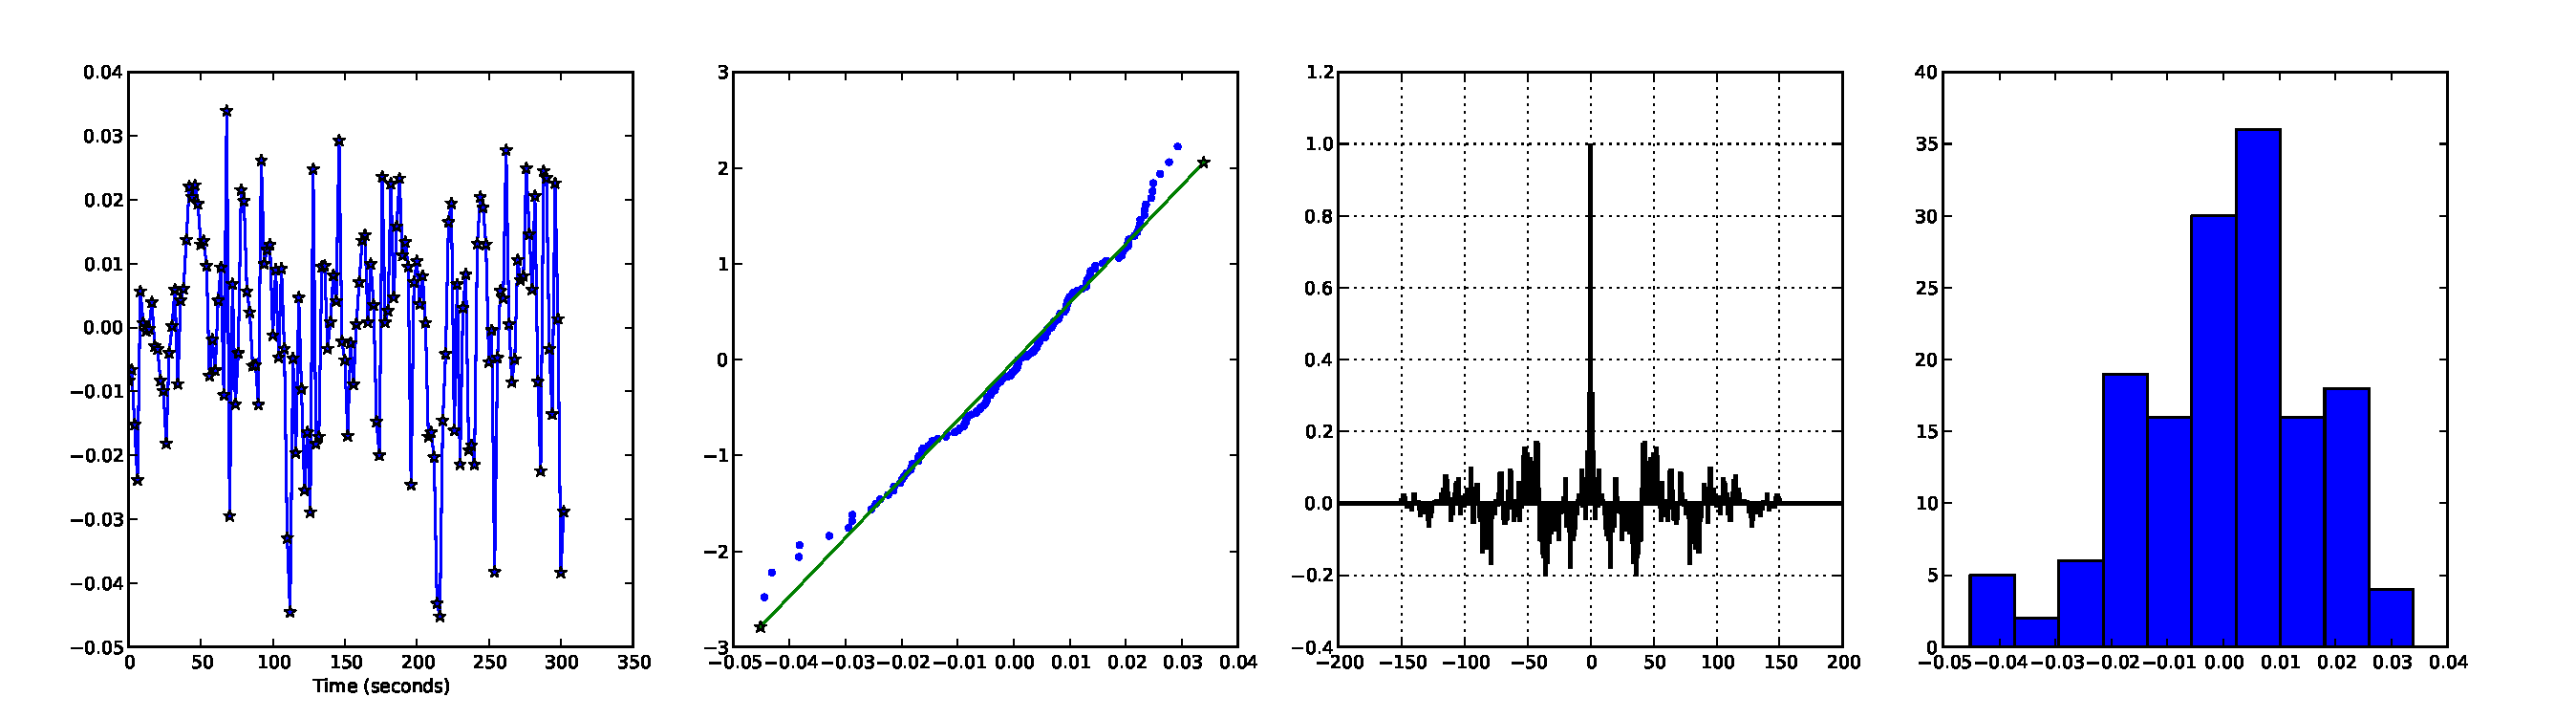
\includegraphics[trim=6cm 1cm 6cm 0cm,width=14cm]{images/noise2_0009s_37_29_24}}
\caption{Q-Q Plots of resting state data, after the de-trending}
\label{fig:QQSpline}
\end{figure}

De-trending the time-series by subtracting a spline fit to the distribution
removed much of the autocorrelation present in \autoref{fig:QQDC:C} and \autoref{fig:QQDC:D},
though clearly not perfectly. Though the distributions still do not exactly fit
the Normal, \autoref{fig:QQs:D} clearly is much improved compared to \autoref{fig:QQDC:D}.
In all, the de-trending is effectively removing Wiener noise. 

\section{Properties of the BOLD Model}
\label{sec:BOLD Analysis}
Since the first complete BOLD model was proposed by \cite{Friston2002}, 
several studies have endeavored to analyze properties of that model. 
The most important property is that the system is dissipative, and given
enough time will converge to a constant value. This is found simply by
analyzing the eigenvalues of the Jacobian of the state equations, 
(\cite{Deneux2006}, \cite{Hu2009}). The steady state of the Balloon
model equations gives:

\begin{eqnarray}
s_{ss} &=& 0 \nonumber \\
f_{ss} &=& \tau_f\epsilon u + 1\nonumber \\
v_{ss} &=& (\tau_f\epsilon u + 1)^\alpha\nonumber \\
q_{ss} &=& \frac{(\tau_f\epsilon u + 1)^\alpha}{E_0}(1-(1-E_0)^{1/(\tau_f\epsilon u + 1)})\nonumber \\
y_{ss} &=& V_0((k_1+k_2)(1-q_{ss}) - (k_2+k_3)(1-v_{ss}))
\label{eq:steadystate}
\end{eqnarray}

In real FMRI data, there is a significant nonlinearity in response; with short sequences
responding disproportionately strong (\cite{Birn2001}, \cite{Wager2005}, \cite{Deneux2006}).
This nonlinearity is accounted for in the Balloon model, although \cite{Deneux2006}
shows that if there will be large variance in the length of signals, 
modeling Neural Habituation may be necessary to fully capture the range of responses. 
Stimuli that last longer than 4 seconds 
tend to be more linear, which is why block designs are so well accounted for
by the General Linear Model (\cite{Birn2001}, \cite{Deneux2006}). For this 
paper we will use only a simple version of the Balloon model, described by
\autoref{eq:bold}, to keep the solution tractable. 

Another interesting result of \cite{Deneux2006} was the sensitivity analysis.
There it was found that many of the parameters compensate for each other,
implying that exact inference of parameters may not be possible without
constraint.

Several studies have been able to calculate distributions for the 
Balloon parameters, those results are summarized in \autoref{tab:Params}

\begin{table}[t]
\centering
\begin{tabular}{|c || c | c | c |}
\hline 
Parameter  & \cite{Friston2002} & \cite{Johnston2008} & \cite{Vakorin2007} \\
\hline
$\epsilon$ &  $N(.54 , .1 ^2)$  & $.069 \pm .014 $ & (NC)\\
$\tau_s  $ &  $N(1.54, .25^2)$  & $4.98 \pm 1.07 $ & $2.2$\\
$\tau_f  $ &  $N(2.46, .25^2)$  & $8.31 \pm 1.51 $ & $.45$\\
$\tau_0  $ &  $N(.98 , .25^2)$  & $8.38 \pm 1.5  $ & $.94$\\
$\alpha  $ &  $N(.33 , .45^2)$  & $.189 \pm .004 $ & $.4$ (NC) \\
$E_0     $ &  $N(.34 , .1 ^2)$  & $.635 \pm .072 $ & $.6$ (NC) \\
$V_0     $ &  $.03$ (NC)        & $.0149 \pm .006$ & (NC)\\
\hline
\end{tabular}
\caption{Parameters found by various studies. (NC) indicates that the value
wasn't calculated. \cite{Vakorin2007} made use of the values from \cite{Friston2002}
where not explicitly stated}
\label{tab:Params} 
\end{table}

Necessary?
[Image with two different $\alpha$'s]
[image comparing the results of 10\% changes in various signals]


